\documentclass[
11pt, % The default document font size, options: 10pt, 11pt, 12pt
%oneside, % Two side (alternating margins) for binding by default, uncomment to switch to one side
openright,
italian, % ngerman for German
singlespacing, % Single line spacing, alternatives: onehalfspacing or doublespacing
%draft, % Uncomment to enable draft mode (no pictures, no links, overfull hboxes indicated)
%nolistspacing, % If the document is onehalfspacing or doublespacing, uncomment this to set spacing in lists to single
%liststotoc, % Uncomment to add the list of figures/tables/etc to the table of contents
%toctotoc, % Uncomment to add the main table of contents to the table of contents
parskip, % Uncomment to add space between paragraphs
%nohyperref, % Uncomment to not load the hyperref package
headsepline, % Uncomment to get a line under the header
%chapterinoneline, % Uncomment to place the chapter title next to the number on one line
%consistentlayout, % Uncomment to change the layout of the declaration, abstract and acknowledgements pages to match the default layout
]{MastersDoctoralThesis} % The class file specifying thse document structure

\usepackage[utf8]{inputenc} % Required for inputting international characters
\usepackage[T1]{fontenc} % Output font encoding for international characters

\usepackage{palatino} % Use the Palatino font by default

\usepackage[backend=bibtex,bibstyle=numeric,citestyle=verbose-ibid]{biblatex} % Use the bibtex backend with the authoryear citation style (which resembles APA)

% Bibliografia
\addbibresource{bibliografia.bib} % The filename of the bibliography
\usepackage[autostyle=true]{csquotes} % Required to generate language-dependent quotes in the bibliography

\newcommand{\virgolette}[1]{``#1''}
% Per l'allineamento delle immagini
\usepackage[export]{adjustbox}

% necessario per risolvere il problema del carattere invisibile per l'a capo
\DeclareUnicodeCharacter{00A0}{ }

% permetti di definire dei colori
\usepackage{xcolor}

% permette di inserire le immagini/tabelle esattamente dove viene usato il
% comando \begin{figure}[H] ... \end{figure}
% evitando che venga spostato in automatico
\usepackage{float}

% permette l'inserimento di url e di altri tipi di collegamento
\usepackage[colorlinks=true]{hyperref}

\hypersetup{
	colorlinks=true, % false: boxed links; true: colored links
	citecolor=black,
	filecolor=black,
	linkcolor=RoyalBlue, % color of internal links
	urlcolor=Maroon  % color of external links
}


% permette al comando \url{...} di andare a capo a metà di un link
\usepackage{breakurl}

% immagini
\usepackage{graphicx}

% permette di riferirsi all'ultima pagina con \pageref{LastPage}
\usepackage{lastpage}

% tabelle su più pagine
\usepackage{longtable}

% per avere dei comandi in più da poter usare sulle tabelle
\usepackage{booktabs}

% tabelle con il campo X per riempire lo spazio rimanente sulla riga
\usepackage{tabularx}

% multirow per tabelle
\usepackage{multirow}

% permette di fare longtable larghe tutta la pagina (parametro x)
\usepackage{tabu}

% imposta lo spazio tra le righe di una tabella
\setlength{\tabulinesep}{6pt}

% personalizza l'intestazione e piè di pagina
%\usepackage{fancyhdr}

% permette di inserire caratteri speciali
\usepackage{textcomp}

% permette di aggiustare i margini e centrare tabelle e figure
\usepackage{changepage}

% Per numerare le tabelle e le figure con la sezione in cui si trovano 
\usepackage{amsmath}
\numberwithin{figure}{section}
\numberwithin{table}{section}

% Use \ul{arg} to undlerline text
\usepackage{soul}

% Per le pagine in orientamento orizzontale
\usepackage{pdflscape}
\usepackage{afterpage}

% Set vertical space in tables
\def\arraystretch{1.5}

% glossary
\usepackage[xindy, acronym]{glossaries}

\definecolor{darkblue}{RGB}{15, 83, 193}
\definecolor{darkgreen}{RGB}{6, 170, 0}
\renewcommand*{\glstextformat}[1]{\textcolor{darkblue}{#1}}

\oddsidemargin=30pt \evensidemargin=20pt%impostano i margini

\setcounter{secnumdepth}{3}


%----------------------------------------------------------------------------------------
%	THESIS INFORMATION
%----------------------------------------------------------------------------------------

\thesistitle{Analisi e personalizzazione di portali B2B} % Your thesis title, this is used in the title and abstract, print it elsewhere with \ttitle
\supervisor{Prof.ssa Ombretta Gaggi} % Your supervisor's name, this is used in the title page, print it elsewhere with \supname
\examiner{} % Your examiner's name, this is not currently used anywhere in the template, print it elsewhere with \examname
\degree{Laurea in Informatica} % Your degree name, this is used in the title page and abstract, print it elsewhere with \degreename
\author{Beatrice Guerra} % Your name, this is used in the title page and abstract, print it elsewhere with \authorname
\addresses{} % Your address, this is not currently used anywhere in the template, print it elsewhere with \addressname

\subject{} % Your subject area, this is not currently used anywhere in the template, print it elsewhere with \subjectname
\keywords{} % Keywords for your thesis, this is not currently used anywhere in the template, print it elsewhere with \keywordnames
\university{Università degli Studi di Padova} % Your university's name and URL, this is used in the title page and abstract, print it elsewhere with \univname
\department{Dipartimento di Matematica \virgolette{Tullio Levi-Civita}} % Your department's name and URL, this is used in the title page and abstract, print it elsewhere with \deptname
\faculty{Corso di Laurea in Informatica} % Your faculty's name and URL, this is used in the title page and abstract, print it elsewhere with \facname

\AtBeginDocument{
	\hypersetup{pdftitle=\ttitle} % Set the PDF's title to your title
	\hypersetup{pdfauthor=\authorname} % Set the PDF's author to your name
	\hypersetup{pdfkeywords=\keywordnames} % Set the PDF's keywords to your keywords
}
%----------------------------------------------------------------------------------------
%	MARGIN SETTINGS
%----------------------------------------------------------------------------------------

\geometry{
	paper=a4paper, % Change to letterpaper for US letter
	inner=2.5cm, % Inner margin
	outer=3.8cm, % Outer margin
	bindingoffset=.5cm, % Binding offset
	top=1.5cm, % Top margin
	bottom=1.5cm, % Bottom margin
%	showframe, % Uncomment to show how the type block is set on the page
}




% Genera automaticamente la pagina di copertina
%\newcommand{\makeFrontPage}{
%  % Declare new goemetry for the title page only.
%  \newgeometry{top=1cm}
%  
%  \begin{titlepage}
%  \begin{center}
%
%  \begin{center}
%  \includegraphics[width=8cm]{../../modello/or-bit_bkg.png}
%  \end{center}
%  
%%  \vspace{1cm}
%
%  \begin{Huge}
%  \textbf{\DocTitle{}}
%  \end{Huge}
%  
%  \textbf{\emph{Gruppo \GroupName{} \, \texttwelveudash{} \, Progetto \ProjectName{}}}
%  
%  \vspace{10pt}
%
%  \bgroup
%  \def\arraystretch{1.3}
%  \begin{tabular}{ r|l }
%    \multicolumn{2}{c}{\textbf{Informazioni sul documento}} \\
%    \hline
%		% differenzia a seconda che \DocVersion{} stampi testo o no
%		\setbox0=\hbox{\DocVersion{}\unskip}\ifdim\wd0=0pt
%			% nulla (non ho trovato come togliere l'a capo)
%			\\
%		\else
%			\textbf{Versione} & \DocVersion{} \\
%		\fi
%    \textbf{Redazione} & \multiLineCell[t]{\DocRedazione{}} \\
%    \textbf{Verifica} & \multiLineCell[t]{\DocVerifica{}} \\
%    \textbf{Approvazione} & \multiLineCell[t]{\DocApprovazione{}} \\
%    \textbf{Uso} & \DocUso{} \\
%    \textbf{Distribuzione} & \multiLineCell[t]{\DocDistribuzione{}} \\
%  \end{tabular}
%  \egroup
%
%  \vspace{10pt}
%
%  \textbf{Descrizione} \\
%  \DocDescription{}  
%
%%  \vspace{0.2cm}
%  
%
%  \end{center}
%  \begin{figure}[H]
%	\includegraphics[height=3cm, right]{../../modello/monolith}
%  \end{figure}
%  \end{titlepage}
%  
%  % Ends the declared geometry for the titlepage
%  \restoregeometry
%}

% -------------------------------------------------------
%  PAGINE INTERNE
% -------------------------------------------------------
%\fancypagestyle{plain}{	
%	% cancella tutti i campi di intestazione e piè di pagina
%	\fancyhf{}
%	\lhead{
%		\includegraphics[height=1.5cm, width=1.5cm, keepaspectratio=true]{../../modello/or-bit_bkg.png}
%		\parbox[b]{10cm}{
%			\emph{\GroupName{}} \vspace{0pt} \\
%			\emph{Progetto \ProjectName{}} \vspace{7pt}
%		}
%	}
%	\chead{}
%	%\rhead{
%	%	\slshape \leftmark
%	%}
%	% Stampa la sezione in alto a destra sull'header
%	\rhead{	
%		\includegraphics[height=1.25cm, width=1.25cm, keepaspectratio=true]{../../modello/monolith}
%	}
%	
%	\lfoot{
%		\DocTitle{} \\
%		% differenzia a seconda che \DocVersion{} stampi testo o no
%		\setbox0=\hbox{\DocVersion{}\unskip}\ifdim\wd0=0pt
%		% nulla
%		\else
%		v \DocVersion{}
%		\fi
%	}
%	\rfoot{Pagina \thepage{} di \pageref{LastPage}}
%	
%	% Visualizza una linea orizzontale in cima e in fondo alla pagina
%	\renewcommand{\headrulewidth}{0.3pt}
%	\renewcommand{\footrulewidth}{0.3pt}
%}
\setlength{\headheight}{30pt}
\pagestyle{plain}

% Per inserire del codice sorgente formattato
\usepackage{listings}
\definecolor{darkgray}{rgb}{.4,.4,.4}
\definecolor{purple}{rgb}{0.65, 0.12, 0.82}
\definecolor{mygreen}{rgb}{0,0.6,0}
\definecolor{mygray}{rgb}{0.5,0.5,0.5}
\definecolor{mymauve}{rgb}{0.58,0,0.82}

\lstset{
	extendedchars=true,          % lets you use non-ASCII characters
	inputencoding=utf8,   % converte i caratteri utf8 in latin1, richiede \usepackage{listingsutf8} anzichè listings
	basicstyle=\ttfamily,        % the size of the fonts that are used for the code
	breakatwhitespace=false,     % sets if automatic breaks should only happen at whitespace
	breaklines=true,             % sets automatic line breaking
	captionpos=b,                % sets the caption-position to top
	commentstyle=\color{mygreen},   % comment style
	frame=none,               % adds a frame around the code
	keepspaces=true,            % keeps spaces in text, useful for keeping indentation of code (possibly needs columns=flexible)
	keywordstyle=\color{blue}\bfseries,     % keyword style
	numbers=none,               % where to put the line-numbers; possible values are (none, left, right)
	numbersep=5pt,              % how far the line-numbers are from the code
	numberstyle=\color{mygray}, % the style that is used for the line-numbers
	rulecolor=\color{black},    % if not set, the frame-color may be changed on line-breaks within not-black text (e.g. comments (green here))
	showspaces=false,           % show spaces everywhere adding particular underscores; it overrides 'showstringspaces'
	showstringspaces=false,     % underline spaces within strings only
	showtabs=false,             % show tabs within strings adding particular underscores
	stepnumber=5,               % the step between two line-numbers. If it's 1, each line will be numbered
	stringstyle=\color{red},    % string literal style
	tabsize=4,                  % sets default tabsize
	firstnumber=1      % visualizza i numeri dalla prima linea
}


\glstoctrue
\makeglossaries
%%%%%%%%%%%%%%%%%%%%%%%%%%%%%%%%%%%%%%%%%%%%%%%%%
%                ACRONIMI
%%%%%%%%%%%%%%%%%%%%%%%%%%%%%%%%%%%%%%%%%%%%%%%%%

\newglossaryentry{IBM}{
	type=\acronymtype, 
	name={IBM}, 
	description={International Business Machines Corporation}, 
	first={IBM},
	see=[Glossary:]{ibmg}
}

\newglossaryentry{ERP}{
	type=\acronymtype, 
	name={ERP}, 
	description={Enterprise Resource Planning}, 
	first={Enterprise Resource Planning (ERP)}, 
	see=[Glossary:]{erpg}
}

\newglossaryentry{IOS}{
	type=\acronymtype, 
	name={iOS}, 
	description={iPhone Operating System}, 
	first={iOS \glsadd{iosg}}, 
	see=[Glossary:]{iosg}
}

\newglossaryentry{B2B}{
	type=\acronymtype, 
	name={B2B}, 
	description={Business-to-Business}, 
	first={B2B \glsadd{b2bg}}, 
	see=[Glossary:]{b2bg}
}

\newglossaryentry{B2C}{
	type=\acronymtype, 
	name={B2C}, 
	description={Business-to-Customer}, 
	first={B2B \glsadd{b2cg}}, 
	see=[Glossary:]{b2cg}
}

\newglossaryentry{CI}{
	type=\acronymtype, 
	name={CI}, 
	description={Customer Intelligence}, 
	first={CI (Customer Intelligence) \glsadd{cig}}, 
	see=[Glossary:]{cig}
}

\newglossaryentry{BI}{
	type=\acronymtype, 
	name={BI}, 
	description={Business Intelligence}, 
	first={BI (Business Intelligence) \glsadd{big}}, 
	see=[Glossary:]{big}
}

\newglossaryentry{CPM}{
	type=\acronymtype, 
	name={CPM}, 
	description={Corporate Performance Management}, 
	first={CPM (Corporate Performance Management) \glsadd{cpmg}}, 
	see=[Glossary:]{cpmg}
}

\newglossaryentry{SEO}{
	type=\acronymtype, 
	name={SEO}, 
	description={Search Engine Optimization}, 
	first={SEO \glsadd{seog}}, 
	see=[Glossary:]{seog}
}

\newglossaryentry{PPC}{
	type=\acronymtype, 
	name={PPC}, 
	description={Pay Per Click}, 
	first={PPC (Pay Per Click) \glsadd{ppcg}}, 
	see=[Glossary:]{ppcg}
}

\newglossaryentry{PMI}{
	type=\acronymtype, 
	name={PMI}, 
	description={Piccole e Medie Imprese}, 
	first={PMI (Piccole e Medie Imprese)}
}

\newglossaryentry{JSF}{
	type=\acronymtype, 
	name={JSF}, 
	description={JavaServer Faces}, 
	first={JSF (JavaServer Faces)},
	see=[Glossary:]{jsfg}
}

\newglossaryentry{CSS}{
	type=\acronymtype, 
	name={CSS}, 
	description={Cascading Style Sheets}, 
	first={CSS}
}

\newglossaryentry{IDE}{
	type=\acronymtype, 
	name={IDE}, 
	description={Integrated Development Environment}, 
	first={IDE},
	see=[Glossary:]{ideg}
}

\newglossaryentry{IVA}{
	type=\acronymtype, 
	name={IVA}, 
	description={Imposta sul Valore Aggiunto}, 
	first={IVA},
	see=[Glossary:]{ivag}
}

\newglossaryentry{API}{
	type=\acronymtype, 
	name={API}, 
	description={Application Programming Interface}, 
	first={API},
	see=[Glossary:]{apig}
}

\newglossaryentry{REST}{
	type=\acronymtype, 
	name={REST}, 
	description={REpresentational State Transfer}, 
	first={REST},
	see=[Glossary:]{restg}
}

\newglossaryentry{SOAP}{
	type=\acronymtype, 
	name={SOAP}, 
	description={Simple Object Access Protocol}, 
	first={SOAP},
	see=[Glossary:]{soapg}
}

\newglossaryentry{CMS}{
	type=\acronymtype, 
	name={CMS}, 
	description={Content Management System}, 
	first={CMS},
	see=[Glossary:]{cmsg}
}

\newglossaryentry{MVC}{
	type=\acronymtype, 
	name={MVC}, 
	description={Model View Controller}, 
	first={MVC (Model View Controller)},
	see=[Glossary:]{mvcg}
}

\newglossaryentry{XHTML}{
	type=\acronymtype, 
	name={XHTML}, 
	description={eXtensible HyperText Markup Language}, 
	first={XHTML},
	see=[Glossary:]{xhtmlg}
}

\newglossaryentry{RTC}{
	type=\acronymtype,
	name={RTC},
	description={Rational Team Concert},
	first={RTC (Rational Team Concert)},
	see=[Glossary:]{rtcg}
}

\newglossaryentry{JSP}{
	type=\acronymtype,
	name={JSP},
	description={JavaServer Pages},
	first={JSP (JavaServer Pages)},
	see=[Glossary:]{jspg}
}

\newglossaryentry{DAO}{
	type=\acronymtype,
	name={DAO},
	description={Data Access Object},
	first={DAO (Data Access Object)},
	see=[Glossary:]{daog}
}

\newglossaryentry{el}{
	type=\acronymtype,
	name={EL},
	description={Expression Language},
	first={Expression Language (EL)},
	see=[Glossary:]{elg}
}

\newglossaryentry{EJB}{
	type=\acronymtype,
	name={EJB},
	description={Enterprise JavaBeans},
	first={Enterprise JavaBeans (EJB)},
	see=[Glossary:]{ejbg}
}

\newglossaryentry{URL}{
	type=\acronymtype,
	name={URL},
	description={Uniform Resource Locator},
	first={URL},
	see=[Glossary:]{urlg}
}

%%%%%%%%%%%%%%%%%%%%%%%%%%%%%%%%%%%%%%%%%%%%%%%%%
%                GLOSSARIO
%%%%%%%%%%%%%%%%%%%%%%%%%%%%%%%%%%%%%%%%%%%%%%%%%

\newglossaryentry{software house}{
	name={software house},
	description={Azienda specializzata principalmente nella produzione di software e applicazioni}
}

\newglossaryentry{ibmg}{
	name={IBM},
	description={Azienda statunitense, tra le maggiori al mondo nel settore informatico. Produce e commercializza hardware e software e servizi informatici, offre infrastrutture, servizi di hosting, servizi di cloud computing e consulenza. Oggi IBM sta emergendo come una società che fornisce soluzioni cognitive e piattaforme cloud}
}

\newglossaryentry{erpg}{
	name={enterprise resource planning},
	description={Enterprise resource planning (letteralmente \virgolette{pianificazione delle risorse d'impresa}, spesso abbreviato in ERP) è un sistema di gestione, chiamato in informatica sistema informativo, che integra tutti i processi di business rilevanti di un'azienda (vendite, acquisti, gestione magazzino, contabilità etc.)}
}

\newglossaryentry{iosg}{
	name={iOS},
	description={Sistema operativo sviluppato da Apple per iPhone, iPod touch e iPad}
}

\newglossaryentry{android}{
	name={Android},
	description={Sistema operativo per dispositivi mobili sviluppato da Google Inc. e basato sul kernel Linux; non è però da considerarsi propriamente un sistema unix-like o una distribuzione GNU/Linux, dato che la quasi totalità delle utilità GNU è sostituita da software in Java}
}

\newglossaryentry{b2bg}{
	name={business-to-business},
	description={Business-to-business, spesso indicato con l'acronimo B2B, in italiano commercio interaziendale, è una locuzione utilizzata per descrivere le transazioni commerciali elettroniche tra imprese, distinguendole da quelle che intercorrono tra le imprese e altri gruppi, come quelle tra una ditta e i consumatori/clienti individuali (B2C, dall'inglese Business to Customer o Business to Consumer, in italiano vendita al dettaglio) oppure quelle tra una impresa e il governo (B2G, dall'inglese Business to Government, lett. "azienda-verso-governo)}
	see=[Glossary:]{b2cg}
}

\newglossaryentry{b2cg}{
	name={business-to-customer},
	description={Con Business-to-customer o Business-to-consumer, spesso abbreviato in B2C, si indicano le relazioni che un'impresa commerciale detiene con i suoi clienti per le attività di vendita e/o di assistenza. Questa sigla è utilizzata soprattutto quando l'interazione tra impresa e cliente avviene tramite internet, ovvero nel caso del commercio elettronico}
}

\newglossaryentry{cig}{
	name={Customer Intelligence},
	description={Il processo di recupero e analisi di informazioni riguardanti i clienti: i loro dettagli e le loro attività, con l'obiettivo di costruire relazioni con il cliente profonde ed solide e di migliorare la strategia di marketing}
}

\newglossaryentry{big}{
	name={Business Intelligence},
	description={Con la locuzione business intelligence (BI) ci si può solitamente riferire a un insieme di processi aziendali per raccogliere dati ed analizzare informazioni strategiche, la tecnologia utilizzata per realizzare questi processi e le informazioni ottenute come risultato di questi processi}
}

\newglossaryentry{cpmg}{
	name={Corporate Performance Management},
	description={Con Corporate Performance Management (CPM) si intende  un insieme di processi per la gestione, la misurazione e il controllo delle performance aziendali, a seguito dell'idinteficazione degli obiettivi da raggiungere in un dato periodo. In tal senso è da considerarsi sinonimo di Business Performance Management (BPM) e Enterprise Performance Management (EPM)}
}

\newglossaryentry{cybersecurity}{
	name={cybersecurity},
	description={Sottoclasse del più ampio concetto di information security. Per cybersecurity si intende infatti quell'ambito dell'information security prettamente ed esclusivamente dipendente dalla tecnologia informatica. Nell'utilizzare il termine cybersecurity si vuole intendere, in particolare, un approccio mirato ad enfatizzare non tanto le misure di prevenzione (ovvero quelle misure che agiscono riducendo la probabilità di accadimento di una minaccia), ma soprattutto le misure di protezione (ovvero quelle misure che agiscono riducendo la gravità del danno realizzato da una minaccia)}
}

\newglossaryentry{Open Power Foundation IBM}{
	name={Open Power Foundation IBM},
	description={La Open Power Foundation è una collaborazione attorno ai prodotti Power Architecture iniziata da IBM e annunciata come l'\virgolette{Open Power Consortium}. L'obiettivo è di permettere ai venditori di ambienti server di costruire server, reti e storage hardware personalizzati per futuri data centers e cloud computing}
}

\newglossaryentry{Beacon Award}{
	name={Beacon Award},
	description={Il programma IBM Beacon Awards premia i Business Partner IBM che offrono soluzioni straordinarie che consentono di ottenere il valore aziendale e trasformare il modo di agire di clienti e settori. I premi del 2017 riconosceranno i risultati conseguiti in una serie di aree di soluzioni – inclusi IBM Watson, Cloud e Analytics – per condurre i clienti nell'era cognitiva}
}

\newglossaryentry{Power}{
	name={Power},
	description={IBM Power Systems è la linea di server basati su tecnologie open e pensati per le applicazioni mission-critical}
}

\newglossaryentry{seog}{
	name={Search Engine Optimization},
	description={Con il termine ottimizzazione per i motori di ricerca (in lingua inglese Search Engine Optimization, in acronimo SEO) si intendono, nel linguaggio di internet, tutte quelle attività volte a migliorare la visibilità di un sito web sui motori di ricerca al fine di migliorare (o mantenere) il posizionamento nelle pagine di risposta alle interrogazioni degli utenti del web. A sua volta, il buon posizionamento di un sito web nelle pagine di risposta dei motori di ricerca è funzionale alla visibilità dei prodotti/servizi venduti}
}

\newglossaryentry{ppcg}{
	name={Pay Per Click},
	description={Il pay per click (PPC) è una modalità di acquisto e pagamento della pubblicità online; l'inserzionista paga una tariffa unitaria in proporzione ai click (click-through rate), ovvero solo quando un utente clicca effettivamente sull'annuncio pubblicitario. Un esempio di pubblicità pay per click è rappresentato dal keyword advertising, cioè annunci sponsorizzati che compaiono a lato dei risultati "puri" dei motori di ricerca}
}

\newglossaryentry{stakeholder}{
	name={Stakeholder},
	description={con il termine stakeholder (o portatore di interesse) si indica genericamente un soggetto (o un gruppo di soggetti) influente nei confronti di un'iniziativa economica, che sia un'azienda o un progetto.
	Fanno, ad esempio, parte di questo insieme: i clienti, i fornitori, i finanziatori come banche e azionisti (o shareholder), i collaboratori, dipendenti ma anche gruppi di interesse locali o gruppi di interesse esterni, come i residenti di aree limitrofe all'azienda e le istituzioni statali relative all'amministrazione locale}
}

\newglossaryentry{jsfg}{
	name={JavaServer Faces},
	description={JavaServer Faces (JSF) è una tecnologia Java, basata sul design pattern architetturale Model-View-Controller (MVC), il cui scopo è quello di semplificare lo sviluppo dell'interfaccia utente (UI) di una applicazione Web; può quindi essere considerata un framework per componenti lato server di interfaccia utente}
}

\newglossaryentry{less}{
	name={Less},
	description={Less è un preprocessore CSS che estende il normale linguaggio CSS permettendo (oltre alla normale sintassi dei fogli di stile) anche l'utilizzo di funzioni, operatori e variabili, la nidificazione delle istruzioni, la creazione di "mixin" e numerose altre caratteristiche che rendono il codice più facile da scrivere, da manutenere e da comprendere}
}

\newglossaryentry{primefaces}{
	name={Primefaces},
	description={PrimeFaces è una suite di componenti open source per la realizzazione dell'interfaccia utente di applicazioni web basate sulla tecnologia Java Server Faces. È sviluppata dalla PrimeTek}
}

\newglossaryentry{eclipse}{
	name={Eclipse},
	description={PrimeFaces è una suite di componenti open source per la realizzazione dell'interfaccia utente di applicazioni web basate sulla tecnologia Java Server Faces. È sviluppata dalla PrimeTek}
}

\newglossaryentry{ideg}{
	name={Integrated Development Environment},
	description={(Ambiente di sviluppo integrato) Strumento software che consiste di più componenti, da cui appunto il nome integrato: un editor di codice sorgente; un compilatore e/o un interprete; un tool di building automatico; un debugger. A volte è integrato anche con un sistema di controllo di versione e uno o più tool per semplificare la costruzione di una GUI}
}

\newglossaryentry{ivag}{
	name={Imposta sul Valore Aggiunto},
	description={Imposta adottata in sessantotto Paesi del mondo (tra i quali anche vari membri dell'UE) applicata sul valore aggiunto di ogni fase della produzione, di scambio di beni e servizi}
}

\newglossaryentry{breadcrumb}{
	name={breadcrumb},
	description={Tecnica di navigazione usata nelle interfacce utente. Il loro scopo è quello di fornire agli utenti un modo di tener traccia della loro posizione in documenti o programmi}
}

\newglossaryentry{tag}{
	name={tag},
	description={Un tag (cioè etichetta, marcatore, identificatore) è una parola chiave o un termine associato a un'informazione (un'immagine, una mappa geografica, un post, un video clip, ecc.), che descrive l'oggetto rendendo possibile la classificazione e la ricerca di informazioni basata su parole chiave}
}

\newglossaryentry{feedback}{
	name={feedback},
	description={Giudizio contenente possibili migliorie e segnalazioni di errori, inviato allo sviluppatore di un'applicazione da un utente che la collauda}
}

\newglossaryentry{wizard}{
	name={wizard},
	description={Procedura informatica, generalmente inglobata in una applicazione più complessa, che permette all'utente di eseguire determinate operazioni (solitamente complesse) tramite una serie di passi successivi}
}

\newglossaryentry{apig}{
	name={API},
	description={Insieme di procedure disponibili al programmatore, di solito raggruppate a formare un set di strumenti specifici per l'espletamento di un determinato compito all'interno di un certo programma. Spesso con tale termine si intendono le librerie software disponibili in un certo linguaggio di programmazione}
}

\newglossaryentry{restg}{
	name={REST},
	description={Architettura software per i sistemi di ipertesto distribuiti come il \textit{World Wide Web}. Il termine REST è spesso usato nel senso di descrivere ogni semplice interfaccia che trasmetta dati su HTTP senza un livello opzionale come \Gls{SOAP}}
}

\newglossaryentry{Magento}{
	name={Magento},
	description={CMS open source per l'e-commerce lanciato il 31 marzo 2008}
}

\newglossaryentry{Prestashop}{
	name={Prestashop},
	description={CMS open source utilizzato per realizzare siti di e-commerce. Nasce nel 2007 e, a differenza dei CMS più \virgolette{generici} diffusi all'epoca della sua prima release (WordPress e Joomla!), Prestashop è interamente pensato per lo sviluppo e la gestione dell'e-commerce.}
}

\newglossaryentry{soapg}{
	name={SOAP},
	description={Protocollo per lo scambio di messaggi tra componenti software, tipicamente nella forma di componentistica software. La parola \textit{object} in \textit{Simple Object Access Protocol} manifesta che l'uso del protocollo dovrebbe effettuarsi secondo il paradigma della programmazione orientata agli oggetti}
}

\newglossaryentry{cmsg}{
	name={Content Management System},
	description={Strumento software, installato su un server web, il cui compito è facilitare la gestione dei contenuti di siti web, svincolando il webmaster da conoscenze tecniche specifiche di programmazione web}
}

\newglossaryentry{mvcg}{
	name={Model View Controller},
	description={Pattern architetturale molto diffuso nello sviluppo di sistemi software, in particolare nell'ambito della programmazione orientata agli oggetti, in grado di separare la logica di presentazione dei dati dalla logica di business}
}

\newglossaryentry{RPG}{
	name={RPG},
	description={Linguaggio di programmazione nativo per minicomputer IBM della serie iSeries, denominata anche, più comunemente, AS/400}
}

\newglossaryentry{AS400}{
	name={AS/400},
	description={Minicomputer sviluppato dall'IBM per usi prevalentemente aziendali, come supporto del sistema informativo gestionale. Attualmente viene utilizzato soprattutto nelle moderne reti di computer come server di applicazioni software, tipicamente di tipo gestionale o comunque di business management, o server di rete (internet/intranet)}
}

\newglossaryentry{xhtmlg}{
	name={XHTML},
	description={Linguaggio di murkup che associa alcune proprietà dell'XML con le caratteristiche dell'HTML: un file XHTML è un pagina HTML scritta in conformità con lo standard XML}
}

\newglossaryentry{framework}{
	name={framework},
	description={Architettura logica di supporto (spesso un'implementazione logica di un particolare design pattern) su cui un software può essere progettato e realizzato, spesso facilitandone lo sviluppo da parte del programmatore}
}

\newglossaryentry{Spring Core}{
	name={Spring Core},
	description={Framework open source per lo sviluppo di applicazioni su piattaforma Java. Esistono numerose estensioni per la costruzione di applicazioni web-based costruite sul modello della piattaforma Java EE}
}

\newglossaryentry{rtcg}{
	name={RTC},
	description={RTC (Rational Team Concert) è uno strumento di collaborazione per lo sviluppo software realizzato da Rational Software, una branca di IBM. Fornisce un ambiente collaborativo che i team di sviluppo utilizzano per gestire tutti gli aspetti legati al loro lavoro (tra cui la pianificazione, i task, il controllo di versione, la gestione della configurazione e i report)}
}

\newglossaryentry{Git}{
	name={Git},
	description={Sistema di controllo di versione per il tracciamento dei cambiamenti nei file e per il coordinamento del lavoro di più persone sugli stessi}
}

\newglossaryentry{Jenkins}{
	name={Jenkins},
	description={Server di automatizzazione open source, aiuta ad automatizzare parti del processo di sviluppo del software tramite integrazione continua}
}

\newglossaryentry{Maven}{
	name={Maven},
	description={Strumento per la compilazione automatizzata usato principalmente per i progetti Java}
}

\newglossaryentry{JavaEE}{
	name={JavaEE},
	description={Enterprise Edition della Java Platform, anche nota come J2EE (Java 2 Enterprise Edition), è una specifica le cui implementazioni vengono principalmente sviluppate in linguaggio di programmazione Java e ampiamente utilizzata nella programmazione Web},
	first={JavaEE (Enterprise Edition)}
}

\newglossaryentry{servlet}{
	name={servlet},
	description={Oggetti scritti in linguaggio Java che operano all'interno di un server web}
}

\newglossaryentry{jspg}{
	name={JavaServer Pages},
	description={Tecnologia di programmazione Web in Java per lo sviluppo della logica di presentazione (tipicamente secondo il pattern MVC) di applicazioni Web, fornendo contenuti dinamici in formato HTML o XML}
}

\newglossaryentry{daog}{
	name={Data Access Object},
	description={Pattern architetturale per la gestione della persistenza: si tratta fondamentalmente di una classe che rappresenta un'entità tabellare di un database relazionale, usata principalmente in applicazioni web per stratificare e isolare l'accesso al data layer da parte della business logic, creando un maggiore livello di astrazione ed una più facile manutenibilità}
}

\newglossaryentry{facelets}{
	name={facelets},
	description={Sistema di template per il web open source, tramite costrutti XML. È la tecnologia utilizzata per creare l'interfaccia utente in JSF}
}

\newglossaryentry{IoC}{
	name={Inversion of Control},
	description={Pattern per cui un componente di livello applicativo riceve il controllo da un componente appartenente a un libreria riusabile. Questo schema ribalta quello tradizionale della programmazione procedurale, dove il codice applicativo svolge i propri compiti richiamando (e quindi passando il controllo a) procedure di libreria},
	first={Inversion of Control (IoC)}
}

\newglossaryentry{elg}{
	name={Expression Language},
	description={Linguaggio di scripting che permette di connettere le pagine JSF al back-end Java}
}

\newglossaryentry{ejbg}{
	name={Enterprise JavaBeans},
	description={Componenti che implementano la logica di business in un'applicazione JavaEE}
}

\newglossaryentry{descrittore di distribuzione}{
	name={descrittore di distribuzione},
	description={File XML che specifica opzioni di configurazione e di contenitore per un'applicazione o un modulo}
}

\newglossaryentry{urlg}{
	name={URL},
	description={Sequenza di caratteri che identifica univocamente l'indirizzo di una risorsa in Internet, tipicamente presente su un host server, come ad esempio un documento, un'immagine o un video, rendendola accessibile ad un client}
}








\begin{document}
	\pagestyle{plain} % Default to the plain heading style until the thesis style is called for the body content
	%----------------------------------------------------------------------------------------
%	TITLE PAGE
%----------------------------------------------------------------------------------------

\begin{titlepage}
	\thispagestyle{empty}
	\begin{center}
		
		\vspace{4cm}
		{\scshape\LARGE \univname}\\\vspace{0.7cm} % University name
		\textsc{\Large \deptname}\\[0.5cm] % Thesis type
		\textsc{\large \facname}
		
		\vspace{2cm}
		\begin{figure}[H]
			\begin{center}
				\includegraphics[height=8cm]{Immagini/logo}
			\end{center}
		\end{figure}
		\vspace{2cm}
		
		
		{\huge \bfseries \ttitle} % Thesis title
		
		\vspace{2cm}
		
		\begin{minipage}[t]{0.49\textwidth}
			\begin{flushleft} \large
				\emph{Relatore} \\
				\supname % Supervisor name
			\end{flushleft}
		\end{minipage}
%
		\begin{minipage}[t]{0.49\textwidth}
			\vspace{1cm}
			\begin{flushright} \large
				\emph{Laureando}\\
				\authorname % Author name
			\end{flushright}
		\end{minipage}
	
		\vspace{1cm}
		{\large Anno accademico 2016-2017}\\[4cm] % Date
		
	\end{center}
\end{titlepage}
	\oddsidemargin=30pt \evensidemargin=20pt%impostano i margini
%	\cleardoublepage
%	\setcounter{page}{1}
	\frontmatter % Use roman page numbering style (i, ii, iii, iv...) for the pre-content pages
	\vspace*{0.2\textheight}

\noindent\enquote{\itshape Ciascuno chiama idee chiare quelle che hanno lo stesso grado di confusione delle sue.}\bigbreak

\hfill Marcel Proust
	
%	\cleardoublepage
	
	%----------------------------------------------------------------------------------------
%	ABSTRACT PAGE
%----------------------------------------------------------------------------------------
\begin{abstract}
	
%\addchaptertocentry{\abstractname} % Add the abstract to the table of contents
In questo lavoro viene analizzato lo sviluppo e l'utilizzo di portali \textit{Business-to-Business}, effettuato durante lo stage svolto presso l'azienda Sanmarco Informatica S.p.A. (Grisignano di Zocco - VI), all'interno della \textit{business unit} 4words. La durata dello stage è stata di 312 ore.\\
L'obiettivo principale da raggiungere era la progettazione e realizzazione di personalizzazioni per portali web esistenti, sulla base di richieste effettuate dai clienti. Obiettivi secondari erano la conoscenza dell'impianto gestionale con cui il portale B2B interagisce, l'autonomia nel rapporto con il cliente stesso e la capacità di redigere analisi e stime per lo sviluppo delle nuove funzionalità richieste.\\
Per svolgere quanto panificato, lo stage si è svolto per l'intera durata in affiancamento, sia in sede che presso clienti. È stata prodotta una sommaria specifica per uno dei progetti seguiti, necessaria per avere una visione d'insieme del progetto, fortemente personalizzato. Sono seguite quindi alcune proposte implementative di nuove richieste, inizialmente svolte in collaborazione e successivamente sviluppate in autonomia.\\
Infine, è stata prodotta una analisi a posteriori di quanto visto, analizzando i vari aspetti caratterizzanti dei portali B2B, sia esternamente, sia internamente all'azienda ospitante.
\end{abstract}
	%----------------------------------------------------------------------------------------
%	ACKNOWLEDGEMENTS
%----------------------------------------------------------------------------------------

\begin{acknowledgements}
\addchaptertocentry{\acknowledgementname} % Add the acknowledgements to the table of contents
The acknowledgments and the people to thank go here, don't forget to include your project advisor\ldots
\end{acknowledgements}

	
	\tableofcontents % Prints the main table of contents
	\listoffigures % Prints the list of figures
	\listoftables % Prints the list of tables
	
%	\clearpage
	
	\mainmatter % Begin numeric (1,2,3...) page numbering
	
	\pagestyle{thesis} % Return the page headers back to the "thesis" style
	
	% Include the chapters of the thesis as separate files from the Chapters folder
	% Uncomment the lines as you write the chapters
	
	\chapter{Introduzione}
\begin{flushright}
	\parbox{13cm}{\small In questo capitolo introduttivo vengono presentati il contesto aziendale in cui si è svolto lo stage e le premesse dello stage stesso. Infine, viene data una panoramica sul contenuto del documento.}
\end{flushright}

\section{L'azienda}
Sanmarco Informatica nasce negli anni '80 come \gls{software house} specializzata nello sviluppo di applicazioni gestionali per aziende manifatturiere ed è oggi una leading company italiana nella progettazione e realizzazione di soluzioni a supporto della riorganizzazione di vari processi aziendali e professionali. L’ambizione e la volontà di rinnovarsi hanno permesso all'azienda di evolversi attraverso esperienze e scelte imprenditoriali di successo, che individuano nella specializzazione del proprio capitale umano l'elemento centrale. L'azienda, partner di \Gls{IBM} Italia, cresce grazie all'impegno di 320 persone fra dipendenti e collaboratori, 13 distributori e 4 sedi – Grisignano di Zocco (VI), Reggio Emilia (RE), Tavagnacco (UD), Vimercate (MB). Le business units Sanmarco Informatica attive sono 5:
\begin{itemize}
	\item \textbf{Jgalileo}: soluzione \Gls{ERP} per diverse tipologie di aziende manifatturiere. Jgalileo costituisce il prodotto di punta dell'azienda, diventando sempre più all'avanguardia grazie all'impegno di oltre 80 consulenti del centro di ricerca e sviluppo software. Questa soluzione gestionale copre le esigenze dell'intero processo aziendale attraverso eccellenze applicative completamente integrate ed è progettato su misura per interpretare al meglio le tipicità di ogni mercato.	
	\item \textbf{4words}: web apps marketing solutions. La web agency sviluppa app \gls{IOS} e \Gls{android} per attività di prevendita, cataloghi prodotti, raccolta ordini, assistenza tecnica, al fine di offrire strumenti sempre più efficaci per la gestione di processi aziendali ERP in mobilità. 4words guida anche il cliente all'utilizzo della piattaforma web a supporto di strategie commerciali \Gls{B2B} e \Gls{B2C}.
	\item \textbf{NextBI}: analizza i dati dei clienti per ottimizzare le strategie di marketing. NextBI vanta infatti grande esperienza in progetti di \gls{CI}, \Gls{BI} e \Gls{CPM}, fornendo moduli già pronti e trasversali a tutti i contesti aziendali.
	\item \textbf{Discovery Quality}: questa suite per la gestione della Qualità, leader di mercato, garantisce al management tutti gli elementi necessari per gestire e misurare la Qualità e le prestazioni, gestendo efficacemente le istanze interne ed esterne di natura etica e sociale.
	\item \textbf{SMItech}: è il Team dedicato alla Tecnologia. L'obiettivo è aiutare i clienti a migliorare sicurezza ed efficienza informatica, attraverso la realizzazione di progetti di infrastruttura IT e lo sviluppo di servizi gestiti di \Gls{cybersecurity}.
\end{itemize}
Sanmarco Informatica è la prima ed unica azienda italiana entrata a far parte dell'\Gls{Open Power Foundation IBM}; a gennaio 2016 l'azienda ha ricevuto il riconoscimento internazionale \Gls{Beacon Award} come finalisti a livello mondiale fra le aziende d'eccellenza che propongono soluzioni tecnologiche innovative in combinazione con il sistema \Gls{Power} di IBM.

\subsection{4words}
4words è una web agency che sviluppa siti web per il business, curandone la realizzazione (web design e criteri di usabilità) e le attività di web – marketing (posizionamento \Gls{SEO}, campagne \Gls{PPC}/AdWords, social media marketing, annunci AdSense, campagne video).
4words realizza inoltre applicazioni per tablet relative al catalogo prodotti, orientate alla vendita, integrabili con siti B2B e B2C e capaci di creare un sistema integrato tra siti e software gestionale Erp.
La capacità di sviluppare applicazioni mobile integrabili con Sistemi Gestionali Erp rende 4words partner ideale per \Gls{PMI} e grandi aziende che vogliano fare un salto tecnologico significativo atto a cogliere potenzialità e vantaggi competitivi del web 2.0 e della connettività mobile.
\paragraph{Realizzazione siti web aziendali} 4words cura la realizzazione e lo sviluppo di siti web aziendali, siti vetrina e catalogo prodotti al fine di far conoscere le realtà commerciali italiane su Internet. La realizzazione di un sito inizia dalla fase di pianificazione del progetto e della strategia da adottare per renderlo user – friendly e facilmente rintracciabile dai motori di ricerca. Successivamente, si passa alla cura della grafica e del design delle pagine. 4words è molto attenta a sviluppare siti web accattivanti e dai contenuti interessanti, al fine di migliorare il business e soddisfare i bisogni del cliente.
\paragraph{Realizzazione siti e-commerce B2C} 4words si occupa della creazione di siti e-commerce per il tuo business realizzando shop online per la vendita di prodotti, basati su ampi database e configuratori semplici da utilizzare e ottimi per visionare e confrontare tutti gli articoli presenti sul sito. Il nostro team cura la realizzazione di e-commerce particolarmente efficaci sia dal punto di vista grafico sia dell'usabilità, affinché l'utente possa consultare rapidamente i prodotti e giungere successivamente al carrello, dove potrà concludere con semplicità l'acquisto.
\paragraph{Realizzazione portali} 4words sviluppa portali B2C atti a contenere grandi quantità di informazioni e ideali per la raccolta dati relativi all'azienda (notizie su blog e forum, documenti consultabili e contenuti scaricabili dall'utente). I portali si rivolgono a tutti gli \gls{stakeholder}, siano essi fornitori, dipendenti o clienti dell'azienda e sono molto utili per i processi decisionali interni all'impresa.
\paragraph{Realizzazione siti business B2B} L'azienda crea e sviluppa siti business B2B, ideali per chi vuole far conoscere la propria azienda su Internet e sviluppare la sua reputazione, grazie a una corretta visibilità sul web.
L'idea è quella di rendere visibili sia le PMI sia le grandi imprese, per realizzare nuove opportunità di business ed essere competitivi sul mercato. 4words adotta le migliori strategie affinché un'azienda sia facilmente rintracciabile sui motori di ricerca e sviluppi fedeltà nel cliente. Un cliente soddisfatto è un cliente che ritorna.

\section{Lo stage}
Lo stage prevedeva l'inserimento nel gruppo web 4words attraverso una prima parte di formazione tramite lezioni frontali e una seconda e più consistente parte in affiancamento, per applicare quanto fino ad ora imparato nel reale contesto aziendale. La durata dello stage è stata di 312 ore, suddivise in 8 settimane. Di queste, 72 ore sono state dedicate alla formazione, e nelle restanti 240 sono state svolte attività di analisi, progettazione e realizzazione di personalizzazioni per i portali web esistenti.

\subsection{Obiettivi}
Gli obiettivi pianificati erano i seguenti:
\begin{table}[h]
	\centering
	\begin{tabular}{|l|}
		\hline
		\textbf{Obbligatori}\\
		\hline
		Progettazione dei portali Web per la raccolta degli ordini \\
		\hline
		Realizzazione software Java \\
		\hline
		Interazione con database SQL \\
		\hline
		Realizzazione front-end HTML, CSS, JavaScript \\
		\hline
		\textbf{Desiderabili}\\
		\hline
		Conoscenza dell'impianto commerciale del gestionale \\
		\hline
		Conoscenza dell'impianto amministrativo del gestionale \\
		\hline
		Autonomia della gestione con il cliente per raccolta nuove richieste \\
		\hline
		\textbf{Opzionali} \\
		\hline
		Analisi e stima nuove richieste clienti \\
		\hline
	\end{tabular}
	
\end{table}
\subsection{Ambiente di lavoro}
Lo stage si è svolto principalmente presso la sede dell'azienda, a Grisignano di Zocco (VI), con qualche uscita presso clienti. All'inizio dello stage mi è stata assegnata la strumentazione necessaria per poter svolgere il lavoro; mi è quindi stato affidato un portatile Lenovo ThinkPad L530, utilizzabile anche nel caso di spostamenti. Nel portatile erano già preinstallati i software di sviluppo utilizzati nell'azienda, tra cui l'\Gls{IDE} \Gls{eclipse}.

%\subsection{Tecnologie utilizzate}
%Le tecnologie utilizzate prevalentemente sono state Java per il back-end, \Gls{JSF} e \Gls{primefaces}, insieme a \acrshort{CSS} e \Gls{less} per il front-end. È stato inoltre utilizzato SQL per l'interfacciamento al database.\footnote{Le tecnologie verranno analizzate successivamente, al capitolo \ref{tecnologie} del presente documento.}

\section{Organizzazione del documento}
Il documento è così strutturato:
\begin{itemize}
	\item Il \textbf{capitolo 2} presenta una analisi del B2B, a livello generale e nel contesto aziendale, analizzando la struttura del progetto, le tecnologie utilizzate, le funzionalità offerte, ed effettuando un confronto con altri contesti presenti nel mercato.
	\item Il \textbf{capitolo 3} descrive quanto svolto durante lo stage nella pratica. Vengono quindi presentati i due progetti interessati, prima a livello generale e poi nello specifico rispetto alle personalizzazioni effettuate.
	\item Nel \textbf{capitolo 4} vengono tratte alcune conclusioni sullo stage svolto, illustrando gli obiettivi raggiunti e le aspettative raccolte al termine dello stage stesso.
\end{itemize}
	\chapter{Il B2B}
\begin{flushright}
	\parbox{13cm}{\small In questo capitolo viene descritto e analizzato il portale B2B, sia a livello generale che nello specifico del contesto aziendale in cui si è svolto lo stage. Vengono analizzate le funzionalità, i fattori di successo e le tecnologie utilizzate, presentandone vantaggi e svantaggi.}
\end{flushright}
\section{Il B2B in generale}
Con B2B si intende un modello per la vendita di prodotti e servizi ad altre aziende. Un portale B2B può essere considerato come un'impresa di supporto che offre ciò di cui le altre aziende necessitano per vincere la concorrenza. Il B2B, infatti, offre prodotti grezzi, servizi o articoli in stock con prezzi molto vantaggiosi rispetto alla usuale vendita al pubblico, in quanto venduti il più delle volte direttamente dalla compagnia che li produce. Al contrario, nei portali B2C destinati al cliente singolo, il prodotto finito viene venduto con un prezzo che rispecchia tutte le piccole transazioni avvenute per la composizione dello stesso: l'azienda A che produce automobili ha dovuto acquistare i bulloni dall'azienda B, le vernici dall'azienda C e il vetro dei finestrini dall'azienda D. Tutti questi acquisti da terzi aumentano di fatto il costo dell'auto finale, che dovrà di per sè garantire la copertura delle spese ed un guadagno per il venditore.

Come qualsiasi altra attività commerciale, il modello B2B richiede una attenta pianificazione. Esso tipicamente fa affidamento su un rapporto solido che il team di vendita instaura con il cliente, mentre quanto inerente la promozione commerciale può includere pubblicità in riviste commerciali, \textit{convention} e conferenze, \textit{marketing} digitale (pubblicità online, tecniche SEO, newsletter) ed altre tecniche di sensibilizzazione tradizionali.

\subsection{Il B2B come e-commerce}
Con la diffusione del web e la rivoluzione digitale, è emerso un nuovo settore definito B2B \textit{e-commerce}. Tramite portali online, le compagnie hanno iniziato a vendere direttamente ad altre aziende, così come a condividere i dati e informazioni riguardo ai prodotti ed ai servizi in modo facile e rapido. Un portale web è infatti sempre raggiungibile e permettete una diffusione immediata
delle informazioni.

Parlando di B2B \textit{e-commerce}, possono essere individuate tre categorie principali:
\begin{description}
	\item[Siti web] Molte aziende necessitano di raggiungere specificatamente altre aziende e i loro impiegati. Il sito web può rappresentare il punto d'entrata di una rete esclusiva riservata ai clienti o agli utenti registrati, o di una rete interna per l'azienda stessa. Le attività possono inoltre vendere direttamente dal sito prodotti che di fatto non richiedono di essere visti dal vivo o provati prima dell'acquisto.
	
	Un esempio sono i B2B che vendono a loro volta B2B, componibili direttamente dal cliente, tramite strumenti di composizione, template, accesso al database, metodologie per le \textit{best practice} e integrazioni per il pagamento.
	
	\item[Fornitura e offerta] Conosciti come \textit{e-procurement}, questi siti sono di solito destinati ad un mercato di nicchia. Un agente può acquistare materiale dal fornitore, richiedere una proposta di vendita ed anche effettuare offerte per comprare ad un prezzo specifico.
	
	I portali delle industrie specializzate o a sviluppo verticale forniscono una sottorete informativa per la specifica industria, come ad esempio le industrie per la sanità, di costruzioni o di altri mercati specifici.
	I portali verticali hanno uno scopo più ampio rispetto ai siti web tradizionali, ma supportano comunque la vendita.
	
	I siti di intermediazione soddisfano i bisogni delle aziende per la fornitura e la richiesta in altro modo: questi siti agiscono come intermediari tra chi fornisce il servizio e il cliente potenziale.
	
	\item[Infomediari] La categoria finale è per i siti informativi, o \virgolette{infomediari}, che forniscono informazioni specializzate per specifiche aziende. Questi portali sono spesso usati come siti organizzativi per gli standard commerciali e industriali.
\end{description}

\subsubsection{Funzionalità base}
Per essere un buon portale, un B2B deve includere alcune funzionalità fondamentali che ne determinano il successo. Queste comprendono ad esempio la gestione dell'ordine, la visualizzazione dei prodotti e la gestione dei clienti. Vi sono poi aspetti legati all'usabilità, come la semplicità nella creazione dell'ordine e l'efficienza nella ricerca di elementi come prodotti o clienti, ed altri inerenti le tecniche SEO.

\paragraph{L'ordine}
L'ordine è l'elemento alla base del B2B. Lo scopo primario di gran parte dei portali B2B è semplificare i processi interaziendali di fornitura e acquisto. L'ordine è anche l'entità più complessa che il B2B gestisce: vi sono infatti moltissimi fattori che dipendono non solo dall'azienda che ne dispone, ma anche dalle leggi statali e continentali in vigore, che possono cambiare anche frequentemente. Si pensi ad esempio all'\Gls{IVA}, una tassa applicata solo in alcuni Paesi, con regole e percentuali differenti. Un buon B2B deve essere in grado, soprattutto se destinato ad un mercato internazionale, o comunque in espansione, di gestire tutte queste variabili, a seconda di dove sta chi vende e chi compra. Non a caso una azienda per la gestione commerciale-amministrativa degli ordini necessita e si avvale di software gestionali, creati appositamente per questo scopo. Il B2B deve quindi essere in grado di riportare le logiche del gestionale nel web, rispettando le convenzioni di quest'ultimo e proponendo delle operazioni \virgolette{guidate}, in modo tale che il sistema sia utilizzabile anche da chi di gestionale ne sa poco o nulla.

\paragraph{Il catalogo}
I prodotti devono essere reperibili ed inseribili in un'ordine. Il loro dettagli deve essere chiaro: un prodotto è sempre caratterizzato da un codice che lo identifica in modo univoco, e che viene spesso utilizzato per acquisti \virgolette{rapidi}, soprattutto quando vengono effettuati ordini ripetuti (un'azienda che utilizza per tutti i macchinari un certo bullone inserirà nell'ordine direttamente il codice, piuttosto che ricercare il prodotto tramite il nome \virgolette{Bullone con testa esagonale m8}).

\paragraph{Caratteristiche generali degli e-commerce}
Essendo un portale destinato agli acquisti, il B2B deve avere le funzionalità base di questa categoria: un carrello per poter raggruppare i prodotti che si vogliono comprare e sapere in anticipo il prezzo totale; un pannello di controllo per il cliente (la \textit{dashboard}) per controllare gli ultimi movimenti e il loro stato; l'accesso al profilo per la modifica di informazioni personali; la possibilità di effettuare il login, fondamentale per poter tenere traccia delle attività svolte dagli utenti. Quest'ultimo fattore svolge un ruolo importante per determinare la strategia di marketing da parte dell'amministrazione.

\paragraph{Filtri e ricerca}
La ricerca di elementi all'interno del portale è una funzionalità che non può mancare, soprattutto con un numero di elementi molto elevato, come spesso avviene nei B2B. Allo stesso modo applicare dei filtri riduce i tempi che l'utente impiega per ottenere ciò che vuole, aumentando di fatto la sua soddisfazione.

\paragraph{Altre funzionalità}
Altre funzionalità che si possono definire \textit{must-have} sono:
\begin{itemize}
	\item configurazione dell'ordine;
	\item informazioni sulla disponibilità e sulla consegna;
	\item prezzo del prodotto pensato sul cliente;
	\item sconti e promozioni;
	\item pagamenti sicuri ed in varie modalità;
	\item \textit{Search Engine Optimization};
\end{itemize}
È necessario inoltre che siano supportati tutti i browser per le versioni più recenti e che le performance del sistema siano buone, sia in termini di caricamento delle pagine, sia per quanto riguarda i tempi di esecuzione di \textit{query} di ricerca nel database.

\subsubsection{I fattori di successo del B2B}
Il commercio \textit{business-to-business} è sempre stato uno dei vantaggi principali per la predominanza delle aziende nella competizione internazionale. L'avvento di Internet e le nuove modalità di commercio e comunicazione hanno però modificato profondamente le dinamiche e i processi tradizionali per tale mercato. Da alcune ricerche sono quindi emersi i fattori critici che una azienda deve considerare per avere successo nel B2B del web: 21 elementi, suddivisi in 5 categorie (strategia di marketing, sito web, dimensione globale, fattori interni e fattori esterni). Per individuarli sono state usate alcune tecniche specifiche, come
\begin{itemize}
	\item scansione ambientale;
	\item analisi della struttura industriale;
	\item opinione di esperti del settore;
	\item analisi della concorrenza;
	\item \textit{best practice};
	\item valutazione interna;
	\item fattori di intuizione;
	\item analisi del profitto di strategie commerciali.
\end{itemize}
Per quanto invece riguarda i fattori proposti, la forza vendita gioca un ruolo centrale nello sviluppo delle strategie di mercato se viene fornita una formazione appropriata. Il coinvolgimento di fornitori e clienti, la cultura del web e l'utilizzo di entrambi i mezzi (tradizionale ed online) sono altri fattori importanti, così come la sicurezza, la fiducia e la confidenza tra il venditore ed il potenziale cliente. L'\textit{e-commerce} è come una relazione tra le parti, dove le alleanze, l'organizzazione e le comunicazioni sono rese possibili dalle nuove tecnologie.

\paragraph{Strategia di marketing}
\subparagraph{Supporto e impegno manageriale}
È richiesta la conoscenza delle potenzialità di Internet da parte del manager, che ha anche il compito di diffonderle in modo proattivo all'interno dell'azienda. L'impegno per il commercio via web aiuta a promuovere il suo sviluppo anche in altre aziende, ma richiede comunque supporto finanziario: c'è un'importante correlazione tra l'investimento effettuato ed il guadagno ottenuto. Per questo il coinvolgimento del livello amministrativo gioca il ruolo più critico.

\subparagraph{Obiettivi strategici}
Il successo dello sviluppo del web B2B dipendono da quanto chiaramente sono definiti gli obiettivi strategici per una organizzazione.

\subparagraph{Integrazione tra Internet e la strategia di marketing}
I responsabili marketing web di successo sono quelli che costruiscono un sistema in grado di integrarsi con le applicazioni esistenti e che possano offrire la formazione necessaria per il suo utilizzo. Sebbene Internet offre molti dei servizi, esso non rimpiazzerà i mezzi tradizionali: i clienti che comprano online continuano comunque a comprare attraverso altri mezzi. Pertanto, le aziende devono considerare il web-marketing come un complemento, piuttosto che un rimpiazzo. Molti clienti infatti preferiscono valutare un prodotto online e poi procedere con l'acquisto in altri modi, di persona o al telefono ad esempio.

\subparagraph{Definizione del target}
Definire chi tra clienti esterni, fornitori, venditori, rivenditori ed altri \textit{business partner} costituisce il target è una operazione primaria, in quanto determina come i canali, gli strumenti e il target stesso sono utilizzati e coinvolti.

\paragraph{Sito web}
\subparagraph{Design}
Un sito web ben progettato e con un bel design è il biglietto da visita dell'azienda nel web. La creazione di un portale richiede però un continuo sforzo per il suo aggiornamento e mantenimento, per continuare a soddisfare le aspettative degli utenti in base alle tendenze. Un ulteriore fattore è il contenuto, che deve essere di valore, accurato ed aggiornato, sia per attrarre nuovi clienti da ogni dove, sia per incoraggiarli a ritornare; le informazioni devono essere chiare e consistenti, in quanto i clienti fanno sempre una valutazione sulla loro utilità nel condurlo a prendere decisioni. La maggior parte degli utenti arriva sul web in cerca di informazioni, pertanto un portale che offre più dettagli sull'azienda e sui prodotti avrà sicuramente più successo. D'altro canto, le performance per l'accesso a tali informazioni sono un dato altrettanto importante: la progettazione del catalogo dei prodotti va sviluppata ancor prima dello stesso portale, in quanto determina la velocità di esecuzione delle \textit{query} di ricerca per migliaia di prodotti.

Vanno quindi considerate tutte le regole base di usabilità, tra cui la semplificazione della navigazione con \gls{breadcrumb} e \gls{tag}, l'interazione e la reattività verso i \gls{feedback} degli utenti, lo scambio di informazioni tra utenti e l'integrazione del web con altri canali di marketing.\virgolette{IL sito web non deve servire solamente come interfaccia di raccolta ordini ma ha anche un alto valore aggiunto per il contenuto informativo}\autocite{b2bSuccessFactors}

\subparagraph{Promozione (offline ed online)}
La promozione è importante per due motivi: il proprio sito web deve essere riconoscibile rispetto a quello della competizione. Questo richiede una alta accessibilità, cosicché sia il sito che la sua pubblicità possano raggiungere il maggior numero di utenti possibile. Secondo, la promozione di un sito web  richiede le conoscenze tecniche di un esperto che sappia come l'utente medio trova usualmente i contenuti su Internet.

\paragraph{Fattori globali}
\subparagraph{Comprensione dell'ambiente esterno}
Un sito dovrebbe rispettare il sistema degli stati in cui è utilizzato. Vanno quindi studiati gli ambienti, incluse le regolazioni del commercio e le modalità di spedizione, per comprendere i vantaggi dei prodotti e dei servizi locali. Il mercato internazionale richiede che vengano effettuate molte considerazioni gestionali e di pianificazione, tra cui lo standard dei prodotti locali, i prezzi di mercato, i fattori competitivi, la valuta, i problemi delle modalità di pagamento, l'assistenza e i servizi offerti ai clienti e considerazioni riguardati le leggi.

\subparagraph{Risorse}
Per essere pronti all'incremento delle vendite che il portale web può portare, sono necessarie risorse, che non tutte le aziende potrebbero avere. Alcuni esempi sono la possibilità di ricevere ordini 24 ore su 24, un servizio clienti efficiente e l'esperienza per la gestione delle spedizioni internazionali

\subparagraph{Multilingua}
Uno dei problemi principali per la comunicazione a livello globale è la lingua. Per le compagnie che vogliono utilizzare il web a livello internazionale, la lingua è la sfida da superare. Per il commercio internazionale è necessario fornire una traduzione per almeno le lingue base, in modo tale da ridurre le difficoltà di comprensione per i lettori non madre-lingua.

\subparagraph{Considerazioni culturali}
Così come la lingua, anche gli altri fattori culturali devono essere riportati nel portale web. Inoltre, fornire informazioni che possano risultare interessanti da una varietà di persone con bisogni e gusti diversi può incoraggiare l'incontro tra le differenti nazioni e culture. Va considerato che anche gli elementi non testuali possono causare incomprensioni culturali, come per esempio l'uso dei colori o dei simboli delle icone (il colore bianco, che in gran parte del mondo è neutrale o addirittura elegante, in alcuni Paesi dell'Asia significa morte).

\subparagraph{Consegna internazionale}
Progettare un sistema logistico in grado di effettuare consegne in più nazioni in modo efficiente è necessario se si vuole vendere in più stati e favorisce la scalabilità per le medie aziende in espansione. Come minimo, quindi, il portale B2B dovrebbe indicare i costi e le tempistiche di spedizione verso tutti i Paesi in cui è disponibile la consegna.

\paragraph{Fattori interni}
\subparagraph{Infrastruttura tecnologica}
Affinché tutto il sistema di cui si è parlato fino ad ora funzioni correttamente, è necessario che l'infrastruttura tecnologica alla base offra buone prestazioni. Questo non è comunque l'unico aspetto da considerare, in quanto Internet per essere uno strumento utile ha bisogno che i suoi utilizzatori abbiano familiarità con il PC e sappiano apprezzare i benefici e le potenzialità che offre.

\subparagraph{Cultura interna}
Un'azienda deve comprendere e abbracciare i nuovi valori, i processi di gestione e gli stili di comunicazione che i nuovi modi di fare marketing creano. Iniziare a commerciare via web è come cominciare in un nuovo stato: la chiave del successo sta nel comprendere, apprezzare e onorare la cultura ed i protocolli di quel paese.

\subparagraph{Forza vendita}
La forza vendita ha un ruolo centrale nel successo di un portale B2B, in quanto in grado di migliorare la comunicazione, aiutando il cliente ad approcciarsi B2B e integrando nuovi strumenti di gestione dell'informazione. Le conoscenze degli addetti al marketing, inoltre, rimangono fondamentali, dato che un sito per quanto tecnologicamente avanzato non può aver successo se non rispetta le aspettative del cliente.

\subparagraph{Formazione}
Una adeguata formazione risulta importante per mantenere aggiornati gli utenti, siano essi interni od esterni, sulle nuove funzionalità e potenzialità delle tecnologie e del sistema.

\paragraph{Fattori esterni}
\subparagraph{Fiducia}
Più l'utente è cosciente di quello che sta facendo nel web, più vorrà delle garanzie. La fiducia verso un sito web sta quindi diventando la chiave che determinerà il successo o il fallimento di molte compagnie. La fiducia è ormai più importante nel monto virtuale che in quello reale, poiché le parti coinvolte in una operazione come può essere l'ordine non sono più nello stesso luogo e di certo non possono dipendere su variabili come la prossimità fisica, la stretta di mano o i segnali del corpo.

\subparagraph{Sicurezza}
Una delle preoccupazioni più diffuse nel web è la sicurezza delle transazioni finanziarie, tanto che alcuni preferiscono guardare i prodotti online, per poi utilizzare metodi offline per confermare l'ordine, come il telefono.

\subparagraph{Relazioni}
I continui cambiamenti che avvengono nel mondo dell'informatica hanno determinato un cambiamento nelle relazioni: esse si basano sempre più sull'informazione che può essere trasmessa tra aziende, piuttosto che sulle modalità con cui questa transazione avviene, come prevede invece la visione tradizionale. Svolgono un ruolo fondamentale quindi i contenuti, le tecnologie e le strategie di marketing.

\subparagraph{Infrastruttura di rete}
Uno dei fattori esterni che non dipendono direttamente dall'azienda è l'infrastruttura di rete: per sfruttare al massimo i vantaggi che il mercato virtuale offre, è necessaria una infrastruttura in grado di supportare le novità che il settore propone. 

\subparagraph{Coinvolgimento del cliente}
Come ultimo punto, ma non meno importante, è il coinvolgimento del cliente in questo tipo di attività. Le aziende dovrebbero impegnarsi a motivare i clienti ad effettuare il passaggio all'ambiente online, oltre che a predisporre un sistema interno in grado di rispondere rapidamente alle richieste dei clienti.
Il modello ottimale che soddisfa a pieno i clienti si basa infatti su una infrastruttura \textit{e-business} con quattro caratteristiche: è facile da usare, ha molte funzionalità, è affidabile ed offre prestazioni elevate.

\section{Il B2B di 4words}
Il B2B di Sanmarco Informatica è un prodotto completo ed al contempo in continua evoluzione. Svolge tutte le funzionalità base che un buon B2B dovrebbe avere e si integra pienamente con gli altri servizi dell'azienda, in particolar modo con il gestionale, agevolando così attività quali l'inserimento e la gestione degli di ordini, la gestione dei documenti e degli appuntamenti, la visualizzazione del catalogo, la configurazione di prodotti. Il B2B è fornito in varie versioni per adattarsi meglio alle esigenze dei clienti:
\begin{itemize}
	\item versione standard (il più diffuso);
	\item versione con web-services;
	\item versione moda.
\end{itemize}
In questa relazione viene trattata solamente la versione standard, l'unica su cui si è incentrato lo stage, mentre verrà solamente presentata la versione con web-services.

\subsection{Funzionalità principali}
In generale, il portale è composto da moduli componibili, in modo tale da essere di per sè un prodotto funzionante, ma anche facilmente personalizzabile secondo le necessità del cliente. I moduli principali sono quello dell'ordine, delle interrogazioni, l'area amministrativa, l'area dei documenti e l'agenda. Tutte queste aree sono attivabili o disattivabili per ogni utente, a seconda del suo gruppo di appartenenza. 

\subsubsection{Abilitazioni e permessi}
Una delle funzionalità principali è infatti la caratterizzazione degli utenti per ruoli. Ad ogni ruolo può essere associata un'abilitazione differente, in modo tale da adattare l'esperienza di navigazione per ognuno di essi. Si considerino per esempio gli amministratori, gli agenti di vendita e i clienti: sono tre tipi di utenza, ai quali però vanno mostrate aree differenti. Gli amministratori possono avere il controllo su tutto, in particolar modo sulle configurazioni. Sono in grado quindi di creare, modificare ed eliminare utenti, bloccarli o sbloccarli, gestire gli ordini, creare, modificare e rimuovere abilitazioni con i relativi permessi, e molto altro. L'amministratore di fatto ha il controllo completo del B2B, può arrivare a qualsiasi area, anche quelle a più basso livello, come la creazione delle connessioni ai database. L'agente di vendita potrebbe invece poter solamente creare ordini, modificandoli fin tanto che non sono inviati, creare e gestire i propri clienti, senza vedere quelli di altri agenti, così come per gli appuntamenti. La navigazione dell'agente è quindi totalmente focalizzata sulla sua funzione all'interno dell'azienda e come nel sistema tradizionale, egli non ha accesso a informazioni riguardanti suoi co-ruolo. Possono fare eccezione i capogruppo, ovvero agenti con un grado di controllo maggiore, che permette loro di controllare le attività dei subordinati. Il ruolo di cliente, infine, è generalmente quello con i permessi minori: il cliente di solito è un'altra azienda o organizzazione, che non deve quindi avere acceso ad informazioni riservate.\\
Le abilitazioni e i permessi sono di fatto del tutto personalizzabili senza l'ausilio di un tecnico 4words. Gli utenti sono inseribili, come visto, in gerarchie, che semplificano ancor di più la gestione da parte dell'amministratore, il quale in pochi passi è in grado di definire regole per molti utenti contemporaneamente. All'utilizzatore finale tutta questa serie di permessi è totalmente trasparente, in quanto non vede che esistono altre aree a lui inaccessibili.

\subsubsection{L'ordine}
Come per ogni B2B, l'ordine rappresenta il fulcro del portale e l'entità più complessa. Per rendere la creazione dell'ordine completa e al tempo stesso \textit{user-friendly}, essa è stata suddivisa in vari step che aiutano l'utente a inserire le informazioni richieste correttamente, presentandogli un numero ridotto di informazioni da fornire e, dove possibile, con aiuti, come ad esempio tramite la scelta multipla (e dunque limitata). Tramite questo \gls{wizard} è quindi possibile inviare ordini, ma anche iniziarli e lasciarli in sospeso per inviarli successivamente.

\subsubsection{Parcheggio}
Una volta inviato, l'ordine può essere inserito direttamente nel gestionale oppure ricevere dei blocchi (amministrativi o commerciali ad esempio), i quali determinano la necessità di approvazione da parte dell'ufficio relativo per il processamento dell'ordine stesso. Questo blocco è detto parcheggio e, con tutte le personalizzazioni possibili in termini di regole e modalità, è un'area molto utile in quanto velocizza alcune operazioni standard. Un tipico esempio di utilizzo è per i clienti fuori fido: a questa categoria viene permesso di fare ordini solamente a certe condizioni, verificate personalmente da alcuni addetti. Ecco quindi che il B2B permette a tali persone di accedere direttamente a tutti gli ordini sottoposti a controllo, sbloccandoli o rifiutandoli con un semplice click, con la possibilità di notificare l'utente di quanto deciso via email. Questa procedura semplifica molto operazioni che fatte direttamente nel gestionale potrebbero risultare non solo più difficoltose, ma anche meno immediate, in quanto per accedere al B2B è sufficiente un tablet o un pc connesso ad internet, mentre il gestionale è solitamente disponibile solamente dentro all'azienda.

\subsubsection{Interrogazioni}
L'area delle interrogazioni è dedicata alla ricerca di schede e informazioni riguardanti i dati inseriti dall'utente. Questi dati possono essere clienti o ordini, e sono suddivisi in varie categorie, così da permettere all'utente di trovare facilmente quello che cerca. In particolare, l'elenco dei clienti creati o utilizzati vengono raccolti in un unica videata, con tutte le loro informazioni. Anche per gli ordini esiste uno storico che indica i dettagli degli ordini inviati, bloccati o sospesi, dove è possibile applicare dei filtri di ricerca, velocizzando molto il procedimento che altrimenti sarebbe stato eseguito nel gestionale.

\subsubsection{Catalogo}
Il catalogo prodotti nella sua versione standard rispetta i requisiti del modello B2B di successo. Esso è presentato in varie modalità, secondo le convenzioni del web, tra cui la visualizzazione a lista (con più dettagli per ogni articolo) e quella a griglia, in cui hanno un ruolo importante le immagini. Questa seconda modalità è di solito rivolta a chi con il proprio B2B vuole rispecchiare gli e-commerce più famosi, come Amazon o Ebay, piuttosto che a clienti che vendono prodotti tecnici di cui sono più importanti le caratteristiche della forma. Il catalogo B2B non solo permette di effettuare ordini secondo le abitudini degli utenti (il 66\% degli utenti di Internet ha fatto acquisti online nel 2016\autocite{eurostat}), ma ha anche la funzione di sostituire i cataloghi stampati che gli agenti di vendita propongono al cliente, in quanto è legato all'utente autenticato ed è una fonte sempre aggiornata. Ad ogni prodotto è possibile associare la disponibilità, aggiornata in tempo reale rispetto al gestionale, riducendo così significativamente il numero di ordini con prodotti non disponibili o non più in produzione. Per l'agente questa è una caratteristica importante, in quanto non è più necessario mettersi in contatto con la sede centrale per conoscere cambiamenti effettuati ai prodotti, anche in termini di prezzi e listini.

\subsection{Struttura del progetto}
Come è strutturato il B2B, sia a livello funzionale, sia a livello progettuale
\subsection{Versionamento}
Come viene versionato
\subsection{Tecnologie utilizzate}
Analisi delle tecnologie utilizzate
\subsubsection{Back-end}
\subsubsection{Front-end} 
%	\chapter{Il B2B}
\begin{flushright}
	\parbox{13cm}{\small In questo capitolo viene descritto e analizzato il portale B2B, sia a livello generale che nello specifico del contesto aziendale in cui si è svolto lo stage. Vengono analizzate le funzionalità, i fattori di successo e le tecnologie utilizzate, presentandone vantaggi e svantaggi.}
\end{flushright}
\section{Il B2B in generale}
Con B2B si intende un modello per la vendita di prodotti e servizi ad altre aziende. Un portale B2B può essere considerato come \textcolor{darkgreen}{uno strumento di supporto che offre ciò di cui un'azienda ha bisogno per vincere la concorrenza} \textcolor{red}{[un'impresa di supporto che offre ciò di cui le altre aziende necessitano per vincere la concorrenza]}. Il B2B, infatti, offre prodotti grezzi, servizi o articoli in stock con prezzi molto vantaggiosi rispetto alla usuale vendita al pubblico, in quanto venduti il più delle volte direttamente dalla compagnia che li produce. Al contrario, nei portali B2C destinati al cliente singolo, il prodotto finito viene venduto con un prezzo che rispecchia tutte le piccole transazioni avvenute per la composizione dello stesso: l'azienda A che produce automobili ha dovuto acquistare i bulloni dall'azienda B, le vernici dall'azienda C e il vetro dei finestrini dall'azienda D. Tutti questi acquisti da terzi aumentano di fatto il costo dell'auto finale, che dovrà di per sè garantire la copertura delle spese ed un guadagno per il venditore.

Come qualsiasi altra attività commerciale, il modello B2B richiede una attenta pianificazione. Esso tipicamente fa affidamento su un rapporto solido che il team di vendita instaura con il cliente, mentre quanto inerente la promozione commerciale può includere pubblicità in riviste commerciali, \textit{convention} e conferenze, \textit{marketing} digitale (pubblicità online, tecniche SEO, newsletter) ed altre tecniche di sensibilizzazione tradizionali.

\subsection{Il B2B come e-commerce}
Con la diffusione del web e la rivoluzione digitale, è emerso un nuovo settore commerciale definito B2B. Tramite portali online, le compagnie hanno iniziato a vendere direttamente ad altre aziende, così come a condividere i dati e informazioni riguardo ai prodotti ed ai servizi in modo facile e rapido. Un portale web è infatti sempre raggiungibile e permettete una diffusione immediata delle informazioni.

Parlando di B2B possono essere individuate tre categorie principali:
\begin{description}
	\item[E-commerce] Molte aziende necessitano di raggiungere specificatamente altre aziende e i loro impiegati. Il sito web può rappresentare il collegamento diretto con una rete esclusiva riservata ai clienti. Le aziende possono inoltre vendere direttamente dal sito prodotti che di fatto non richiedono di essere visti dal vivo o provati prima dell'acquisto. Un esempio sono i B2B che vendono a loro volta B2B, componibili direttamente dal cliente tramite editor, \textit{template} e vari plugin per le più svariate funzionalità.
	
	\item[Fornitura e offerta] Questi siti sono di solito destinati ad un mercato di nicchia. Un agente può acquistare materiale dal fornitore, richiedere una proposta di vendita ed anche effettuare offerte per comprare ad un prezzo specifico. È in questa categoria che ricade il B2B \textcolor{darkgreen}{della \textit{business unit}} 4words.
	
	\item[Informativi] La categoria finale è per i siti informativi, che forniscono informazioni specializzate per determinati settori. Questi portali sono spesso usati come siti organizzativi per gli standard commerciali e industriali.
\end{description}

\subsubsection{Funzionalità base}
Per essere un buon portale, un B2B deve includere alcune funzionalità fondamentali che ne determinano il successo. Queste comprendono ad esempio la gestione dell'ordine, la visualizzazione dei prodotti e la gestione dei clienti. Vi sono poi aspetti legati all'usabilità, come la semplicità nella creazione dell'ordine e l'efficienza nella ricerca di elementi come prodotti o clienti, ed altri inerenti le tecniche SEO.

\paragraph{L'ordine}
L'ordine è l'elemento alla base del B2B. Lo scopo primario di gran parte dei portali B2B è semplificare i processi interaziendali di fornitura e acquisto. 

L'ordine è anche l'entità più complessa che il B2B gestisce: vi sono infatti moltissimi fattori che dipendono non solo dall'azienda che ne dispone, ma anche dalle leggi statali e continentali in vigore, che possono cambiare anche frequentemente. Si pensi ad esempio all'\Gls{IVA}, una tassa applicata solo in alcuni Paesi, con regole e percentuali differenti.

Un buon B2B deve essere in grado, soprattutto se destinato ad un mercato internazionale, o comunque in espansione, di gestire tutte queste variabili, a seconda di dove sta chi vende e chi compra. Non a caso un'azienda per la gestione commerciale-amministrativa degli ordini necessita e si avvale di software gestionali, creati appositamente per questo scopo. Il B2B deve quindi essere in grado di riportare le logiche del gestionale nel web, rispettando le convenzioni di quest'ultimo e proponendo delle operazioni \virgolette{guidate}, in modo tale che il sistema sia utilizzabile anche da chi di gestionale ne sa poco o nulla.

\paragraph{Il catalogo}
I prodotti devono essere reperibili ed inseribili in un ordine. Il loro dettaglio deve essere chiaro: un prodotto è sempre caratterizzato da un codice che lo identifica in modo univoco e che viene spesso utilizzato per acquisti \virgolette{rapidi}, soprattutto quando vengono effettuati ordini ripetuti (un'azienda che utilizza per tutti i macchinari un certo bullone inserirà nell'ordine direttamente il codice \virgolette{BX123Y}, piuttosto che ricercare il prodotto tramite la stringa \virgolette{Bullone con testa esagonale m8}).

\paragraph{Caratteristiche generali degli e-commerce}
Essendo un portale destinato agli acquisti, il B2B deve avere le funzionalità base di questa categoria: un carrello per poter raggruppare i prodotti che si vogliono comprare e sapere in anticipo il prezzo totale; un pannello di controllo per il cliente (la \textit{dashboard}) per tenere traccia degli ultimi movimenti e del loro stato; l'accesso al profilo per la modifica di informazioni personali; la possibilità di effettuare il login, fondamentale per controllare le attività svolte dagli utenti.

\paragraph{Filtri e ricerca}
La ricerca di elementi all'interno del portale è una funzionalità che non può mancare, soprattutto con un numero di elementi molto elevato, come spesso avviene nei B2B. Allo stesso modo applicare dei filtri riduce i tempi che l'utente impiega per ottenere ciò che vuole, aumentando di fatto la sua soddisfazione.

\paragraph{Altre funzionalità}
Altre funzionalità che si possono definire \textit{must-have} sono:
\begin{itemize}
	\item configurazione dell'ordine;
	\item informazioni sulla disponibilità e sulla consegna;
	\item prezzo del prodotto pensato sul cliente;
	\item sconti e promozioni;
	\item pagamenti sicuri ed in varie modalità;
	\item \textit{Search Engine Optimization};
\end{itemize}
È necessario inoltre che siano supportati tutti i \textit{browser} per le versioni più recenti e che le performance del sistema siano buone, sia in termini di caricamento delle pagine, sia per quanto riguarda i tempi di esecuzione di \textit{query} di ricerca nel database.

\subsubsection{I fattori di successo del B2B}
Il commercio \textit{business-to-business} è sempre stato uno dei vantaggi principali per la predominanza delle aziende nella competizione internazionale. L'avvento di Internet e \textcolor{darkgreen}{i nuovi modi di comunicare} \textcolor{red}{[le nuove modalità di commercio e comunicazione]} hanno però modificato profondamente le dinamiche \textcolor{red}{[e i processi tradizionali]} per tale mercato. \textcolor{darkgreen}{Si è cercato quindi di analizzare i fattori che determinano il successo delle aziende nell'ambito del B2B \textit{e-commerce}} \textcolor{red}{[Da alcune ricerche sono quindi emersi i fattori critici che un'azienda deve considerare per avere successo in questo settore: 21 elementi, suddivisi in 5 categorie (strategia di marketing, sito web, dimensione globale, fattori interni e fattori esterni)]}: per individuarli sono state usate alcune tecniche specifiche, come
\begin{itemize}
	\item scansione ambientale;
	\item analisi della struttura industriale;
	\item opinione di esperti del settore;
	\item analisi della concorrenza;
	\item \textit{best practice};
	\item valutazione interna;
	\item fattori di intuizione;
	\item analisi del profitto.
\end{itemize}
\textcolor{darkgreen}{Ne sono emerse cinque categorie (strategia di marketing, sito web, dimensione globale, fattori interni e fattori esterni) a cui il portale B2B realizzato deve saper adattarsi.}
\textcolor{red}{[Per quanto invece riguarda i fattori proposti, la forza vendita gioca un ruolo centrale nello sviluppo delle strategie di mercato se viene fornita una formazione appropriata. Il coinvolgimento di fornitori e clienti, la cultura del web e l'utilizzo di entrambi i mezzi (tradizionale ed online) sono altri fattori importanti, così come la sicurezza, la fiducia e la confidenza tra il venditore ed il potenziale cliente.]}

\paragraph{Strategia di marketing}
\textcolor{darkgreen}{I primi fattori determinanti per il successo del portale costituiscono una precondizione alla realizzazione dello stesso. In particolare, il \textbf{supporto da parte dei manager}, sia ideale che finanziario, la \textbf{definizione di obiettivi e del target} e l'\textbf{integrazione con i sistemi tradizionali} in uso rendono la successiva realizzazione del B2B efficace ed efficiente. Queste condizioni facilitano anche il rapporto tra le due aziende legate dal B2B, quella che lo vende e quella che lo utilizza, in quanto definiscono informazioni importanti per l'analisi e la progettazione del portale. Più sono precise e definite le precondizioni, più è preciso il preventivo che ne scaturisce, con il risultato di un portale B2B che soddisfa a pieno le esigenze dell'azienda usufruente.}

\textcolor{darkgreen}{Una nota particolare va posta sull'utilizzo del web come strumento commerciale: sebbene esso offra tutto ciò di cui il mercato necessita, compresa la sicurezza dei pagamenti (l'argomento più delicato in questo ambito), ancora non è stato in grado di rimpiazzare i metodi tradizionali di vendita: molti clienti preferiscono infatti utilizzare i B2B (ma anche gli altri \textit{e-commerce}) per valutare i prodotti, per poi procedere all'acquisto \virgolette{di persona} o telefonicamente. Rimane quindi ancora fondamentale il rapporto tra venditore e acquirente.}

\textcolor{red}{\textbf{Supporto e impegno manageriale}
	È richiesta la conoscenza delle potenzialità di Internet da parte del manager, che ha anche il compito di diffonderle in modo proattivo all'interno dell'azienda. L'impegno preso verso il commercio nel web aiuta a promuovere il suo sviluppo anche in altre aziende, ma richiede comunque supporto finanziario: c'è un'importante correlazione tra l'investimento effettuato ed il guadagno ottenuto. Per questo il coinvolgimento del livello amministrativo gioca il ruolo più critico.}
	
\textcolor{red}{\textbf{Obiettivi strategici}
	Il successo dello sviluppo del web B2B dipende da quanto chiaramente sono definiti gli obiettivi strategici per una organizzazione.}
	
\textcolor{red}{\textbf{Integrazione tra Internet e la strategia di marketing}
	I responsabili marketing web di successo sono quelli che, oltre a costruire un sistema in grado di integrarsi con le applicazioni esistenti, sappiano offrire la formazione necessaria per il suo utilizzo. Sebbene Internet offra molti dei servizi comuni, esso non rimpiazzerà i mezzi tradizionali: i clienti che comprano online continuano comunque a comprare attraverso altri mezzi. Pertanto, le aziende devono considerare il web-marketing come un complemento, piuttosto che un rimpiazzo. Molti clienti infatti preferiscono valutare un prodotto online e poi procedere con l'acquisto in altri modi, di persona o al telefono ad esempio.}
	
\textcolor{red}{\textbf{Definizione del target}
	Definire chi tra clienti esterni, fornitori, venditori, rivenditori ed altri \textit{business partner} costituisce il target di vendita è una operazione primaria, in quanto determina come i canali, gli strumenti e il target stesso vadano utilizzati e coinvolti.}

\paragraph{Sito web}
\textcolor{darkgreen}{Il B2B è un sito web. Da ciò derivano una serie di regole che richiedono impegno e risorse per essere rispettate, ma che portano vantaggi in termini di visibilità ed apprezzamento, il successo appunto. Essendo il biglietto da visita dell'azienda, il B2B deve quindi essere ben progettato e con un bel design.}
	
\textcolor{darkgreen}{La creazione di un portale richiede però un continuo sforzo di aggiornamento e mantenimento, per soddisfare le aspettative degli utenti. La maggior parte di questi arriva sul web in cerca di informazioni, pertanto un B2B che offre più dettagli sull'azienda e sui prodotti avrà sicuramente più successo di uno in cui i prodotti sono meno caratterizzati. D'altro canto, le performance per l'accesso a tali informazioni sono un dato altrettanto importante: per questo motivo la progettazione del catalogo prodotti va realizzata ancor prima dello stesso portale, in quanto determina la velocità di esecuzione delle \textit{query} di ricerca per migliaia di elementi.}
	
\textcolor{darkgreen}{Vanno quindi considerate tutte le regole base di usabilità, tra cui la semplificazione della navigazione con \gls{breadcrumb} e \gls{tag}, lo scambio di informazioni tra utenti e l'integrazione del B2B con altri canali di marketing.}

\textcolor{red}{\textbf{Design}
Un sito web ben progettato e con un bel design è il biglietto da visita dell'azienda nel web. La creazione di un portale richiede però un continuo sforzo per il suo aggiornamento e mantenimento, per continuare a soddisfare le aspettative degli utenti in base alle tendenze. Un ulteriore fattore è il contenuto, che deve essere di valore, accurato ed aggiornato, sia per attrarre nuovi clienti da ogni dove, sia per incoraggiarli a ritornare; le informazioni devono essere chiare e consistenti, in quanto i clienti fanno sempre una valutazione sulla loro utilità nel condurlo a prendere decisioni.}

\textcolor{red}{Vanno quindi considerate tutte le regole base di usabilità, tra cui la semplificazione della navigazione con \gls{breadcrumb} e \gls{tag}, l'interazione e la reattività verso i \gls{feedback} degli utenti, lo scambio di informazioni tra utenti e l'integrazione del web con altri canali di marketing. \virgolette{Il sito web non deve servire solamente come interfaccia di raccolta ordini ma ha anche un alto valore aggiunto per il contenuto informativo}\autocite{bib:b2bSuccessFactors}.}

\textcolor{red}{\textbf{Promozione (offline ed online)}
La promozione è importante per due motivi: il proprio sito web deve essere riconoscibile rispetto a quello della competizione. Questo richiede un'alta accessibilità, cosicché sia il sito che la sua pubblicità possano raggiungere il maggior numero di utenti possibile. Secondo, la promozione di un sito web  richiede le conoscenze tecniche di un esperto che sappia come l'utente medio trova usualmente i contenuti su Internet.}

\paragraph{Fattori globali}
\textcolor{darkgreen}{Uno degli obiettivi del B2B (e delle aziende che lo vogliono) è quello di ampliare l'area geografica di vendita. Spesso le aziende adottano il portale B2B per espandersi all'estero, dove magari hanno più mercato per la tipologia di prodotti che vendono. Questa espansione richiede alcune caratteristiche importanti nel B2B, non sempre scontate da implementare, tra cui:
\begin{itemize}
	\item rispetto delle convenzioni e delle regolazioni commerciali vigenti nei vari Paesi (es.: valuta, tipi di pagamento, tasse e dazi);
	\item multilingua;
	\item utilizzo di icone significative e comprensibili a livello globale;
	\item integrazione con i servizi di consegna internazionale;
\end{itemize}}

\textcolor{red}{\textbf{Comprensione dell'ambiente esterno}
Un sito dovrebbe rispettare il sistema degli stati in cui è utilizzato. Vanno quindi studiati gli ambienti, incluse le regolazioni del commercio e le modalità di spedizione, per comprendere i vantaggi dei prodotti e dei servizi locali. Il mercato internazionale richiede che vengano effettuate molte considerazioni gestionali e di pianificazione, tra cui lo standard dei prodotti locali, i prezzi di mercato, i fattori competitivi, la valuta, i problemi delle modalità di pagamento, l'assistenza, i servizi offerti ai clienti e considerazioni riguardanti le leggi locali.}

\textcolor{red}{\textbf{Risorse}
Per essere pronti all'incremento delle vendite che il portale web può portare, sono necessarie risorse che non tutte le aziende potrebbero avere. Alcuni esempi sono la possibilità di ricevere ordini 24 ore su 24, un servizio clienti efficiente e l'esperienza per la gestione delle spedizioni internazionali.}

\textcolor{red}{\textbf{Multilingua}
Uno dei problemi principali per la comunicazione a livello globale è la lingua. Per le compagnie che vogliono utilizzare il web a livello internazionale, la lingua è la sfida da superare. Per il commercio internazionale è necessario fornire una traduzione per almeno le lingue base, in modo tale da ridurre le difficoltà di comprensione per i lettori non madre-lingua.}

\textcolor{red}{\textbf{Considerazioni culturali}
Così come la lingua, anche gli altri fattori culturali devono essere riportati nel portale web. Inoltre, fornire informazioni che possano risultare interessanti da una varietà di persone con bisogni e gusti diversi può incoraggiare l'incontro tra le differenti nazioni e culture. Va considerato che anche gli elementi non testuali possono causare incomprensioni culturali, come per esempio l'uso dei colori o dei simboli delle icone (il colore bianco, che in gran parte del mondo è neutrale o addirittura elegante, in alcuni Paesi dell'Asia significa morte).}

\textcolor{red}{\textbf{Consegna internazionale}
Progettare un sistema logistico in grado di effettuare consegne in più nazioni efficientemente è necessario se si vuole vendere in più stati e favorisce la scalabilità per le medie aziende in espansione. Come minimo, quindi, il portale B2B dovrebbe indicare i costi e le tempistiche di spedizione verso tutti i Paesi in cui è disponibile la consegna.}

\paragraph{Fattori interni}
\textcolor{darkgreen}{Per quanto bene possa essere realizzato, i portali B2B, compreso quello di 4words, necessitano di alcuni requisiti per l'utilizzo. In particolare, l'infrastruttura tecnologica in cui l'applicativo viene installato deve avere caratteristiche hardware discrete e il personale incaricato alla gestione deve essere in grado di utilizzarlo. Per questo secondo fattore, solitamente vengono organizzati corsi di formazione e dimostrazioni sia dall'azienda che lo produce, sia internamente all'azienda che lo utilizza, per fornire una panoramica delle funzionalità ai responsabili e agli agenti, la forza vendita delle aziende. Sono poi questi che portano e iscrivono nuovi clienti.}

\textcolor{red}{\textbf{Infrastruttura tecnologica}
Affinché tutto il sistema di cui si è parlato fino ad ora funzioni correttamente, è necessario che l'infrastruttura tecnologica alla base offra buone prestazioni. Questo non è comunque l'unico aspetto da considerare, in quanto Internet per essere uno strumento utile ha bisogno che i suoi utilizzatori abbiano familiarità con il PC e sappiano apprezzare i benefici e le potenzialità che esso offre.}

\textcolor{red}{\textbf{Cultura interna}
Un'azienda deve comprendere e abbracciare i nuovi valori, i processi di gestione e gli stili di comunicazione che i nuovi modi di fare marketing creano. Iniziare a commerciare via web è come trasferirsi in un nuovo stato: la chiave del successo sta nel comprendere, apprezzare e onorare la cultura ed i protocolli di quel Paese.}

\textcolor{red}{\textbf{Forza vendita}
La forza vendita ha un ruolo centrale nel successo di un portale B2B, in quanto in grado di migliorarne l'espressività, aiutando il cliente ad approcciarsi al portale e integrando nuovi strumenti di gestione dell'informazione. Le conoscenze degli addetti al marketing, inoltre, rimangono fondamentali, dato che un sito per quanto tecnologicamente avanzato non può aver successo se non rispetta le aspettative del cliente.}

\textcolor{red}{\textbf{Formazione}
Una adeguata formazione risulta importante per mantenere aggiornati gli utenti, siano essi interni o esterni, sulle nuove funzionalità e potenzialità del sistema.}

\paragraph{Fattori esterni}
\textcolor{darkgreen}{Il successo del B2B dipende anche da alcuni fattori esterni, che possono non derivare direttamente dalla sua implementazione, come la fiducia tra le parti (fornitore e acquirente), la sicurezza di operazioni come i pagamenti, la relazione con la tecnologia dei clienti ed il coinvolgimento di questi nell'utilizzo del portale.}

\textcolor{darkgreen}{In conclusione, il modello di B2B ottimale che soddisfa a pieno i clienti ha quattro caratteristiche: è facile da usare, ha molte funzionalità, è affidabile ed offre prestazioni elevate.}

\textcolor{red}{\textbf{Fiducia}
Più l'utente è cosciente di quello che sta facendo nel web, più vorrà delle garanzie. La fiducia verso un sito web sta quindi diventando la chiave che determinerà il successo o il fallimento di molte compagnie. La fiducia è ormai più importante nel mondo virtuale che in quello reale, poiché le parti coinvolte in operazioni come l'ordine non sono più nello stesso luogo e di certo non possono dipendere su variabili come la prossimità fisica, la stretta di mano o i segnali del corpo.}

\textcolor{red}{\textbf{Sicurezza}
Una delle preoccupazioni più diffuse nel web è la sicurezza delle transazioni finanziarie, tanto che alcuni preferiscono guardare i prodotti online, per poi utilizzare i metodi tradizionali per effettuare i pagamenti.}

\textcolor{red}{\textbf{Relazioni}
I continui cambiamenti che avvengono nel mondo dell'informatica hanno determinato un cambiamento nelle relazioni: esse si basano sempre più sull'informazione che può essere trasmessa tra aziende, piuttosto che sulle modalità con cui questa transazione avviene, come prevede invece la visione tradizionale. Svolgono un ruolo fondamentale quindi i contenuti, le tecnologie e le strategie di marketing.}

\textcolor{red}{\textbf{Infrastruttura di rete}
Uno dei fattori esterni che non dipendono direttamente dall'azienda è l'infrastruttura di rete: per sfruttare al massimo i vantaggi che il mercato virtuale offre, è necessaria un'infrastruttura in grado di supportare le novità che il settore propone. }

\textcolor{red}{\textbf{Coinvolgimento del cliente}
Come ultimo punto, ma non meno importante, è il coinvolgimento del cliente in questo tipo di attività. Le aziende dovrebbero impegnarsi a motivare i clienti ad effettuare il passaggio all'ambiente online, oltre che a predisporre un sistema interno in grado di rispondere rapidamente alle richieste dei clienti.
Il modello ottimale che soddisfa a pieno i clienti si basa infatti su una infrastruttura \textit{e-business} con quattro caratteristiche: è facile da usare, ha molte funzionalità, è affidabile ed offre prestazioni elevate.}

\section{Il B2B di 4words}
Il B2B di Sanmarco Informatica è un prodotto completo ed al contempo in continua evoluzione. Svolge tutte le funzionalità base che un buon B2B dovrebbe avere e si integra pienamente con gli altri servizi dell'azienda, in particolar modo con il gestionale, agevolando così attività quali l'inserimento e la gestione degli ordini, la gestione dei documenti e degli appuntamenti, la visualizzazione del catalogo \textcolor{darkgreen}{e} la configurazione di prodotti. Il B2B è fornito in varie versioni per adattarsi meglio alle esigenze dei clienti:
\begin{itemize}
	\item versione standard (il più diffuso);
	\item versione con web-services;
	\item versione moda.
\end{itemize}
In questa relazione viene trattata solamente la versione standard, l'unica su cui si è incentrato lo stage, mentre verrà solamente presentata la versione con web-services.

Ogni B2B venduto è personalizzato, anche solo in minima parte, secondo le richieste del cliente. È raro dunque incontrare due portali identici, poiché per quanto essi possano assomigliarsi per forma e contenuti, vi sono sempre delle funzionalità da una parte che l'altra ha, per scelta del cliente, nascoste.
Esistono versioni molto basilari, in cui viene personalizzato solamente l'aspetto o, ad esempio, il menu, ed altre in cui ritrovare lo standard è quasi un'impresa. Molto spesso l'utilizzo sempre più massivo del portale fa sì che sorgano proposte da parte dell'utilizzatore, che vede nel B2B la soluzione per snellire alcune pratiche altrimenti richiedenti l'uso del gestionale.

\subsection{Funzionalità principali}
In generale, il portale è composto da moduli componibili, in modo tale da essere di per sè un prodotto funzionante, ma anche facilmente personalizzabile secondo le necessità del cliente. I moduli principali sono quello dell'ordine, delle interrogazioni, l'area amministrativa, l'area dei documenti e l'agenda. Tutte queste aree sono attivabili o disattivabili per ogni utente, a seconda del suo gruppo di appartenenza. 

\subsubsection{Abilitazioni e permessi}
Una delle funzionalità principali è infatti la caratterizzazione degli utenti per ruoli. Ad ogni ruolo può essere associata un'abilitazione differente, in modo tale da adattare l'esperienza di navigazione per ognuno di essi. Si considerino per esempio gli amministratori, gli agenti di vendita e i clienti: sono tre tipi diversi di utenza, ai quali vanno mostrate aree differenti. Gli amministratori possono avere il controllo su tutto, in particolar modo sulle configurazioni. Sono in grado quindi di creare, modificare ed eliminare utenti, bloccarli o sbloccarli, gestire gli ordini, creare, modificare e rimuovere abilitazioni con i relativi permessi, e molto altro.

L'amministratore di fatto ha il controllo completo del B2B, può arrivare a qualsiasi area, anche quelle a più basso livello, come la creazione delle connessioni ai database.

L'agente di vendita potrebbe invece poter solamente creare ordini, modificandoli fin tanto che non sono inviati, creare e gestire i propri clienti, senza vedere quelli di altri agenti, così come per gli appuntamenti. La navigazione dell'agente è quindi totalmente focalizzata sulla sua funzione all'interno dell'azienda e, come nel sistema tradizionale, egli non ha accesso a informazioni riguardanti suoi co-ruolo. Possono fare eccezione i capogruppo, ovvero agenti con un grado di controllo maggiore, che permette loro di controllare le attività dei subordinati.

Il ruolo di cliente, infine, è generalmente quello con i permessi minori: il cliente di solito è un'altra azienda o organizzazione, che non deve quindi avere acceso ad informazioni riservate.

Le abilitazioni e i permessi sono di fatto del tutto personalizzabili senza l'ausilio di un tecnico 4words. Gli utenti sono inseribili, come visto, in gerarchie, che semplificano ancor di più la gestione da parte dell'amministratore, \textcolor{darkgreen}{che} \textcolor{red}{[il quale]} in pochi passi è in grado di definire regole per molti utenti contemporaneamente. All'utilizzatore finale tutta questa serie di permessi è totalmente trasparente, in quanto non vede che esistono altre aree a lui inaccessibili.

\subsubsection{L'ordine}
Come per ogni B2B, l'ordine rappresenta il fulcro del portale e l'entità più complessa. Per rendere la creazione dell'ordine completa e al tempo stesso \textit{user-friendly}, essa è stata suddivisa in vari step che aiutano l'utente a inserire le informazioni richieste correttamente, presentandogli un numero ridotto di informazioni da fornire e, dove possibile, con aiuti, come ad esempio la scelta multipla (e dunque limitata). Tramite questo \gls{wizard} è quindi possibile inviare ordini, ma anche iniziarli e lasciarli in sospeso per inviarli successivamente.

\subsubsection{Parcheggio}
Una volta inviato, l'ordine può essere inserito direttamente nel gestionale oppure ricevere dei blocchi (amministrativi o commerciali ad esempio), i quali determinano la necessità di approvazione da parte dell'ufficio relativo per il suo processamento. Questo blocco è detto parcheggio e, con tutte le personalizzazioni possibili in termini di regole e modalità, è un'area molto utile in quanto velocizza alcune operazioni standard. Un tipico esempio di utilizzo è per i clienti fuori fido: a questa categoria viene permesso di fare ordini solamente a certe condizioni, verificate personalmente da alcuni addetti. Ecco quindi che il B2B permette a tali persone di accedere direttamente a tutti gli ordini sottoposti a controllo, sbloccandoli o rifiutandoli con un semplice click, con la possibilità di notificare l'utente di quanto deciso via email. Questa procedura semplifica molto operazioni che fatte direttamente nel gestionale potrebbero risultare non solo più difficoltose, ma anche meno immediate, in quanto per accedere al B2B è sufficiente un tablet o un pc connesso ad internet, mentre il gestionale è solitamente disponibile solamente dentro all'azienda.

\subsubsection{Interrogazioni}
L'area delle interrogazioni è dedicata alla ricerca di schede e informazioni riguardanti i dati inseriti dall'utente. Questi dati sono suddivisi in varie categorie, così da permettere all'utente di trovare facilmente quello che cerca. In particolare, l'elenco dei clienti viene raccolto in un 'unica videata, con tutte le loro informazioni. Anche per gli ordini esiste uno storico che ne indica i dettagli, dove è possibile applicare dei filtri, velocizzando molto il procedimento di ricerca.

\subsubsection{Catalogo}
Il catalogo prodotti nella sua versione standard rispetta i requisiti del modello B2B di successo. Esso è presentato in varie modalità, secondo le convenzioni del web, tra cui la visualizzazione a lista (con più dettagli per ogni articolo) e quella a griglia, in cui hanno un ruolo importante le immagini. Questa seconda modalità è di solito rivolta a chi con il proprio B2B vuole rispecchiare gli e-commerce più famosi, come Amazon o Ebay, piuttosto che a clienti che vendono prodotti tecnici di cui sono più importanti le caratteristiche della forma.

Il catalogo B2B non solo permette di effettuare ordini secondo le abitudini degli utenti (il 66\% degli utenti di Internet ha fatto acquisti online nel 2016\autocite{bib:eurostat}), ma ha anche la funzione di sostituire i cataloghi stampati che gli agenti di vendita propongono al cliente, in quanto è legato all'utente autenticato ed è una fonte sempre aggiornata.

Ad ogni prodotto è possibile associare la disponibilità, aggiornata in tempo reale rispetto al gestionale, riducendo così significativamente il numero di ordini con prodotti non disponibili o non più in produzione. Per l'agente questa è una caratteristica importante, in quanto non è più necessario mettersi in contatto con la sede centrale per conoscere cambiamenti effettuati ai prodotti, anche in termini di prezzi e listini.

\subsection{Struttura del progetto}
Passando agli aspetti implementativi, il B2B di 4words è strutturato gerarchicamente in vari progetti, con in testa alla gerarchia la versione base e al di sotto varie versioni dipendenti dalle soprastanti. In particolare la versione standard precedentemente citata è così formata:
\begin{itemize}
	\item B2B Base: costituisce gran parte del back-end dell'applicazione. Contiene pressoché tutta la logica del portale e non ha alcun tipo di riferimento al front-end. Si occupa principalmente di gestire i dati del gestionale, riproducendoli sotto forma di oggetti.
	\item B2B Prime: è il nucleo del front-end. Include le librerie grafiche e predispone la totalità delle pagine navigabili nel portale. Si occupa anche di collegare il front-end alle classi del back-end, aggiungendo o aggiustando gli oggetti per renderli usufruibili dalla parte grafica.
	\item B2B R14: costituisce l'ultima grossa release di creazione del portale e rappresenta l'ultimo strato comune a tutti i progetti. È il vero e proprio applicativo ed in esso vengono definiti i denominatori comuni per creare uno standard stabile e duraturo, oltre che compatibile con i molti moduli disponibili per l'installazione.
\end{itemize}
Questi tre progetti formano quello che si è soliti definire lo standard del B2B. Esso rende l'installazione per il cliente semplice e immediata in quanto configura già di suo la maggior parte delle funzionalità.
Da questi tre progetti si sviluppano poi una serie di moduli tra loro indipendenti, tra cui:
\begin{itemize}
	\item B2B TCE: è il modulo che integra il B2B con il configuratore di prodotto offerto dall'azienda.
	\item B2B Rest Service: include le librerie necessarie per interrogare le \Gls{API} di servizi \Gls{REST}, come ad esempio di \Gls{Magento} o \Gls{Prestashop}. È il ponte tra il B2B e i vari \Gls{CMS} disponibili online e il suo scopo è proprio quello di agevolare l'interfacciamento tra questi due tipi di contenuto.
	\item B2B Rest Client: costituisce l'interfaccia grafica dell'integrazione B2B con i servizi web.
\end{itemize}
A partire da questi progetti vengono quindi creati i prodotti finali venduti ai clienti. Ogni cliente ha il suo progetto dedicato, in quanto sorgono in continuazione nuove richieste, sviluppate quindi in un ambiente indipendente, in modo tale da non creare conflitti con implementazioni contrarie di altri clienti.

Il B2B è strutturato secondo il pattern \Gls{MVC}. Questo pattern è individuabile in più livelli:
\begin{itemize}
	\item Nell'architettura ad alto livello, il \textit{model} è composto dai componenti che contengono la logica dell'applicazione, in particolare da \textit{manager}, \textit{data provider} e \textit{program provider}; la \textit{view} è composta dal \virgolette{codice JSF}; il controller è costituito dalla FacesServlet, una \gls{servlet} che gestisce le richieste delle applicazioni web \textcolor{darkgreen}{e inizializza le risorse richieste\footnote{Maggiori dettagli sulla servlet utilizzata da JSF sono forniti in \hyperref[app:javaee]{appendice \ref{app:javaee}}}. Uno schema di questo pattern è rappresentato in \hyperref[fig:mvc-arch]{figura \ref{fig:mvc-arch}}\autocite{bib:jsf-mvc}}.
	\item La view del precedente livello rispecchia a sua volta il pattern, dove il \textit{model} è costituito dalle entità, la \textit{view} è composta dalle pagine \texttt{\gls{XHTML}} (le \gls{facelets}) e il controller è formato dai \textit{backing bean}.
\end{itemize}
L'architettura può quindi essere riassunta con lo schema M(MVC)C. Questa ricorsione si potrebbe protrarre anche al livello del client, aggiungendo quindi un ulteriore livello interno.
\begin{figure}
	\centering
	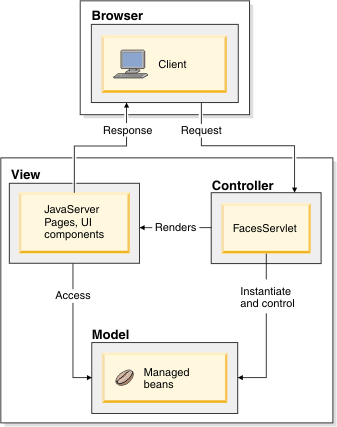
\includegraphics{Immagini/mvc-jsf.png}
	\caption{Pattern MVC a livello architetturale}
	\label{fig:mvc-arch}
\end{figure}

Nel B2B il \textit{model} architetturale è stato suddiviso in vari \textit{package}, citati precedentemente. I \textit{manager} contengono la logica dell'applicazione e collegano la \textit{view} ai \textit{data provider}, i quali rappresentano il \textit{data layer} nel pattern architetturale \Gls{DAO}. Questi, inoltre, possono fare riferimento al loro interno ai \textit{program provider}, i quali rappresentano l'interfaccia Java per i programmi \Gls{RPG} dell'\Gls{AS400}. Secondo le norme di programmazione prestabilite per il progetto B2B, dunque, il flusso esecutivo per una operazione che richiede la chiamata ad un programma RPG è il seguente: la pagina fa riferimento ad un metodo del \textit{backing bean}, che chiama il manager di competenza, il quale trasferisce la richiesta al \textit{data provider}, che richiama il \textit{program provider}. Il risultato della chiamata al programma torna quindi indietro attraverso \textit{data provider}, \textit{manager} e \textit{backing bean}, che effettueranno eventuali controlli e operazioni necessari. Infine, se richiesto dall'applicativo, la pagina viene aggiornata e/o nuovamente renderizzata.

Quasi la totalità delle entità concepite nel B2B 4words ha un oggetto corrispettivo nei \textit{backing bean}, nei \textit{manager}, nei \textit{data provider} e, a volte, nei \textit{program provider}. Questa suddivisione permette di applicare il \textit{single responsibility principle} (principio di singola responsabilità), secondo il quale ogni elemento deve avere una singola responsabilità, interamente incapsulata dall'elemento stesso. Ad esempio, l'entità \texttt{Order} è gestita rispettivamente nell'\texttt{OrderBck} per quanto riguarda il suo interfacciamento con le pagine JSF, nell'\texttt{OrderManager} per la logica e nell'\texttt{OrderDataProvider} per l'accesso al database. Anche le personalizzazioni risultano così immediate, in quanto, per la gerarchia descritta precedentemente, è sufficiente derivare la classe che richiede la personalizzazione per usufruire di tutti i vantaggi che la struttura porta con sé, tra cui il polimorfismo.

Le pagine \texttt{XHTML} sono strutturate in modo tale da permettere il riutilizzo ove possibile, tramite template e componenti creati ad hoc per svolgere alcuni compiti specifici, come il calendario o il campo di testo per la valuta. Questo è reso possibile anche grazie all'utilizzo di JSF.

\subsubsection{Vantaggi e svantaggi}
La struttura appena descritta presenta alcuni vantaggi e svantaggi importanti.
\paragraph{Vantaggi}
Il primo vantaggio è che la suddivisione in più progetti permette che essi siano gestiti da un gruppo limitato di persone, riducendo il rischio di creare conflitti nelle modifiche contemporanee. Inoltre, ogni progetto cliente è indipendente dagli altri e dipende solo dai pacchetti di cui necessita: non vengono installate librerie al di fuori di quelle richieste per il corretto funzionamento, mantenendo quanto si va ad installare il più leggero possibile.

La separazione in più progetti permette anche una distribuzione dei ruoli all'interno del gruppo di sviluppo: l'implementazione di nuove funzionalità generali e solitamente di grosso impatto è affidata al gruppo standard; la personalizzazione delle funzionalità esistenti e lo sviluppo di funzionalità specifiche o non comuni, che quindi risulterebbero utili a pochi, è lasciato ai sistemisti con a carico il cliente. Nel caso in cui sorgano anomalie o problematiche negli ambienti dei clienti riguardo a moduli standard, interviene l'assistenza, la quale si occupa di individuare e correggere gli errori cosicché possa essere rilasciato un aggiornamento risolutivo comune per tutti i clienti.

La struttura gerarchica fortemente basata sull'ereditarietà facilita anche chi si addentra per la prima volta in un progetto così ampio nell'individuare il flusso d'esecuzione. I passaggi e le chiamate tra metodi seguono infatti sempre la stessa linea: pagina, \textit{backing bean}, \textit{manager}, \textit{data provider}, \textit{program provider} e ritorno.

\paragraph{Svantaggi}
Uno degli svantaggi principali nell'utilizzo di questa struttura è che con aggiornamenti del pacchetto standard importanti, laddove il cliente ha un portale molto personalizzato, c'è il rischio che le personalizzazioni si invalidino, richiedendo di fatto un lungo lavoro di \virgolette{riporto} delle classi personalizzate per mantenerle compatibili con la nuova versione standard. Vi sono di fatto due possibilità: aggiornare l'intero pacchetto standard e modificare di conseguenza la parte personalizzata o procedere al contrario, aggiornando solamente ciò che aggiunge funzionalità o che corregge comportamenti anomali, senza modificare i metodi standard richiamati dalle classi personalizzate. Nel primo caso, come detto, il lavoro può risultare molto lungo, mentre nel secondo caso si rischia di arrivare ad uno stato di inconsistenza, dove più classi richiedono che uno stesso metodo svolga operazioni diverse, dovendo quindi comunque effettuare modifiche a svariate personalizzazioni. Tutto questo prevede anche una lunga fase di test, ai quali non viene mai dedicato il giusto tempo.

\subsection{Versionamento}
Lo strumento di versionamento utilizzato per tutti i progetti riguardanti il B2B è \Gls{RTC}. Esso si basa su IBM Jazz, una piattaforma estendibile che aiuta i team ad integrare i task durante il ciclo di vita del software. RTC è costruito su una architettura client-server ed è integrabile con molti altri prodotti, tra cui \gls{Git}, \Gls{Jenkins} e \Gls{Maven}. Per quanto riguarda la funzione di versionamento, RTC è così strutturato: sul server sono presenti gli \textit{stream}, dei contenitori per uno o più progetti, accessibili solamente tramite invito. Agli utenti invitati vengono attribuiti uno o più ruoli, ad esempio \textit{scrum master} o membro del team (solitamente lo sviluppatore), che determinano i permessi a loro associati. 

RTC è strutturato secondo lo schema in \hyperref[fig:rtc-struttura]{figura \ref{fig:rtc-struttura}}\autocite{bib:rtcDoc}.
\begin{figure}
	\centering
	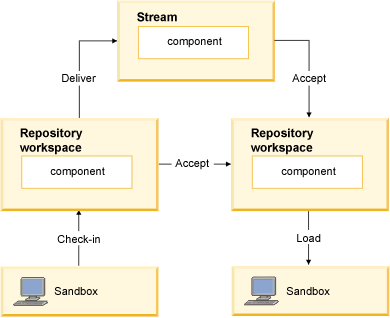
\includegraphics{Immagini/rtc-struttura.png}
	\caption{Struttura del sistema di versionamento RTC}
	\label{fig:rtc-struttura}
\end{figure}
Il sistema è centralizzato sullo \textit{stream}, sul quale confluiscono tutte le modifiche e dal quale gli utenti scaricano i progetti. Vi è poi un livello intermedio, appartenente ai singoli utenti, che si trova sul server e permette agli utenti di salvare le proprie modifiche online, così da non correre il rischio di perderle a causa di malfunzionamenti hardware. Questo strato è chiamato \textit{repository workspace}. Infine, il livello più basso è quello che risiede in locale, nel PC in cui si lavora. Le operazioni tra livelli hanno nomi specifici: il \textit{check-in} è il trasferimento delle modifiche dal \textit{workspace} locale a quello remoto; con \textit{deliver} si intende il trasferimento delle modifiche dal \textit{workspace} remoto allo \textit{stream}. Con questa operazione le modifiche diventano effettive e scaricabili da tutti gli utenti, i quali devono accettarle (\textit{accept}) per trasferirle al proprio \textit{workspace} remoto e quindi riportarle in ambiente locale tramite l'operazione \textit{load}.

Le funzionalità principali di RTC utilizzate per lo sviluppo del B2B sono:
\begin{itemize}
	\item \textit{work item}: sono il meccanismo sui cui si basa RTC per tracciare e coordinare i \textit{task} di sviluppo e il flusso di lavoro. Sono il collegamento tra varie funzionalità di RTC, come le \textit{build} e i \textit{change set} (l'insieme delle modifiche associate, appunto, al \textit{work item}). I \textit{work item} possono assumere una categoria diversa a seconda del loro contesto, come ad esempio \virgolette{implementazione} o \virgolette{bug}, per distinguere se le modifiche rilasciate costituiscono una nuova implementazione o risolvono una anomalia presente nel codice.
	\item Controllo dei sorgenti: è un sistema di controllo di versione costruito sulla piattaforma Jazz. Offre supporto per lo sviluppo parallelo con modello agile, integrando anche un sistema di gestione degli errori.
	\item Pianificazione: il componente per la pianificazione fornisce uno strumento di assistenza nell'organizzazione e svolgimento di progetti agile e non. Per lo sviluppo agile permette di salvare lo stato dei lavori ad una certa \textit{release} o ad uno \textit{sprint} e di tenere traccia del progresso durante le iterazioni, bilanciando il lavoro tra gli sviluppatori. Questo modello viene utilizzato soprattutto per lo sviluppo dei progetti standard, in quanto le personalizzazioni sono solitamente affidate ad una o due persone.
\end{itemize}
RTC è usato tramite la sua integrazione per Eclipse, l'IDE di sviluppo del B2B. Un tipico esempio di utilizzo di RTC è presentato in \hyperref[fig:rtc]{figura \ref{fig:rtc}}\autocite{bib:rtcDoc}.
\begin{figure}
	\centering
	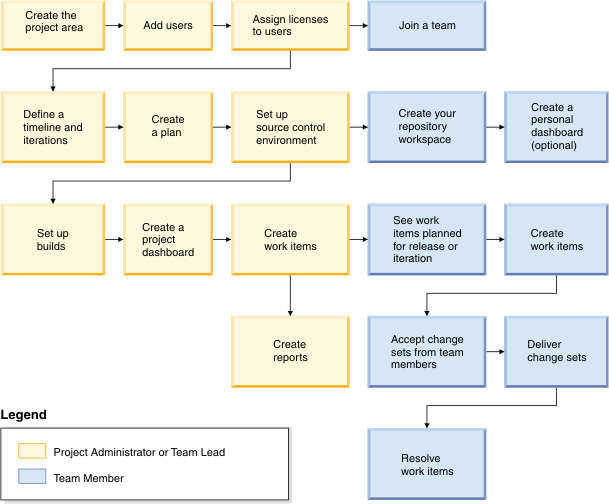
\includegraphics[width=14cm]{Immagini/rtc-task-flow.png}
	\caption{Flusso di lavoro tipico di RTC}
	\label{fig:rtc}
\end{figure}

\subsubsection{Vantaggi e svantaggi}
Per analizzare i vantaggi e gli svantaggi di questo strumento, viene fatto un confronto con Git.
\paragraph*{Modello di repository}
\begin{itemize}
	\item[\textbf{Git}:] distribuito. I vari \textit{repository} agiscono come peer e gli utenti hanno solitamente una copia locale con tutta la storia dei cambiamenti in aggiunta a quella in cui stanno lavorando.
	\item[\textbf{RTC}:] \textit{client-server}. Gli utenti accedono ad un \textit{repository} principale (lo \textit{stream}) tramite un \textit{client}; tipicamente in locale viene conservata solamente la copia di lavoro del progetto e i cambiamenti devono essere inviati allo \textit{stream} prima di essere propagati agli altri utenti.
\end{itemize}
Il vantaggio che un sistema centralizzato ha rispetto ad uno distribuito è che lo spazio richiesto per mantenere in locale la copia del progetto è limitato alle sole dimensioni dei file dello stesso. Questo comporta però la necessità di essere collegati in rete anche solo per consultare le modifiche apportate ad un file, che non sono disponibili in locale. Questo comportamento presenta anche il seguente svantaggio: se per un progetto di un cliente lo standard rilasciato non è aggiornato con le ultime modifiche presenti sullo \textit{stream}, un nuovo componente del team che dovrà lavorare su quel progetto scaricherà una versione diversa da quella del cliente. Non c'è pertanto la sicurezza che quanto modificato funzioni effettivamente, se non aggiornando il pacchetto standard interamente, operazione rischiosa se fatta da tale nuova persona, che può non conoscere approfonditamente tutte le personalizzazioni del cliente.

Per ovviare a questo problema sono possibili varie strategie: la prima è un passaggio manuale del \textit{workspace} locale del progetto tra lo sviluppatore che si è occupato del cliente in questione e il nuovo arrivato. Questo, oltre a non essere sempre possibile, presenta alcuni problemi: nel caso in cui non si voglia aggiornare tutto il pacchetto standard del cliente con la versione corrente dello \textit{stream}, ma solo con alcune modifiche (correttive ad esempio), diventa necessario comunicare agli altri detentori del progetto quali work item sono stati scaricati o che modifiche sono state fatte, in modo tale che possano essere riportate in tutte le versioni locali. Una operazione simile è del tutto contraria alle logiche e alle regole dei sistemi di versionamento. La seconda opzione è quella di creare nello \textit{stream} dei clienti una copia dei progetti standard, cosicché ogni progetto cliente sia indipendente. Questa strategia richiede però un impegno maggiore, soprattutto in termini di manutenibilità. Una ulteriore possibilità è quella di creare delle \textit{release} per i vari progetti clienti, in modo tale che il nuovo componente possa scaricare lo \textit{stream} standard alla \textit{release} del cliente. Questa andrà revisionata man mano che vengono effettuati gli aggiornamenti. Lo svantaggio di questa modalità è che nello \textit{stream} del progetto standard emergono tante \textit{release} quanti sono i clienti e, per numero molto ampio, potrebbe appesantire lo \textit{stream} stesso. Nonostante ciò, quest'ultima strategia sembra essere la più idonea per gestire questo genere di situazioni.

\paragraph*{Gestione della concorrenza}
\begin{itemize}
	\item[\textbf{Git}:] \textit{merge}. Le modifiche possono avvenire in modo concorrente e l'utente è avvisato di possibili conflitti quando vuole eseguire un aggiornamento del \textit{repository}. Questo conflitto può essere risolto direttamente dal sistema o manualmente dall'utente per poi inviare la nuova versione agli utenti.
	\item[\textbf{RTC}:] \textit{merge} o \textit{lock}. Sebbene sia disponibile anche il modello \textit{lock}, in cui le modifiche non sono permesse finché l'utente non chiede e riceve il \textit{lock} esclusivo sul file, per il B2B è utilizzato il sistema di \textit{merge}, come in Git.
\end{itemize}
La scelta di utilizzare il modello di \textit{merge} è sicuramente la migliore, in quanto permette di collaborare contemporaneamente sugli stessi file, il che rappresenta un notevole vantaggio nello sviluppo dei progetti.

\paragraph*{Metodo di salvataggio}
\begin{itemize}
	\item[\textbf{Git}:] \textit{snapshot}. Vengono salvati per ogni versione i file interi, compressi per ottimizzare e ridurre la dimensione complessiva dell'albero.
	\item[\textbf{RTC}:] \textit{change set}. Vengono salvati solamente i cambiamenti tra revisioni.
\end{itemize}
Sebbene con il modello di salvataggio utilizzato da Git le varie versioni dei file sono accessibili in modo immediato, il modello a \textit{change set} richiede di fatto meno spazio sul disco. Nello specifico, nello sviluppo del B2B risulta più un vantaggio questo risparmio rispetto al tempo di accesso a revisioni precedenti. 

\paragraph*{Integrazione con gli IDE}
\begin{itemize}
	\item[\textbf{Git}:] ampio supporto. 
	\item[\textbf{RTC}:] Eclipse e Visual Studio.
\end{itemize}
L'ampio supporto che gli IDE offrono verso Git rappresenta un grosso svantaggio per RTC, il quale offre \textit{plug-in} solamente per Eclipse e Visual Studio. Nel caso di utilizzo di altri ambienti, quindi, questo sistema di versionamento non è utilizzabile.

\subsection{Tecnologie utilizzate}
L'intero B2B è sviluppato sulla piattaforma \Gls{JavaEE}. In particolare sono utilizzati Java e il \textit{framework} Spring per il \textit{back-end}, JSF e Primefaces per il \textit{front-end}. Apache Tomcat è invece il contenitore \gls{servlet} \textit{open source} utilizzato come piattaforma di esecuzione per il portale. Esso non può essere definito un \textit{application server} in quanto non implementa la specifica JavaEE, ma solamente il supporto verso servlet e \Gls{JSP}.

\subsubsection{Ambiente di sviluppo}
L'ambiente di sviluppo utilizzato per il B2B è Eclipse. Questo strumento, sebbene sia \textit{open source}, non è immediato come l'IDE da me utilizzato in ambiente universitario, IntelliJ. La principale differenza rilevata nell'utilizzo di questi due strumenti è la capacità di interpretare il contesto. IntelliJ è di gran lunga più \virgolette{intelligente} e in grado di facilitare il programmatore nel suo lavoro. Eclipse è invece molto più statico e funzionalità come il completamento o il debug risultano complessivamente meno rapide ed intuitive. Gli unici svantaggi di IntelliJ rispetto ad Eclipse sono che il primo è a pagamento nella sua versione Ultimate, non supporta RTC e per fornire funzionalità avanzate come quelle che effettivamente offre, richiede caratteristiche hardware maggiori per l'esecuzione. Complessivamente, tra i due continuo a ritenere IntelliJ molto più avanzato.

\subsubsection{Back-end}
Il \textit{back-end} del B2B è sviluppato in Java. Questo rappresenta un vantaggio soprattutto per il contesto di sviluppo, il B2B. Essendo strettamente legato ad un sistema gestionale, è istintivo pensare ad oggetti. In particolare, se combinato al gestionale Galileo offerto dall'azienda, questa caratteristica emerge maggiormente. Per quanto riguarda l'aspetto web, l'utilizzo della JavaEE permette di creare applicazioni portabili e scalabili, in grado di interfacciarsi con tecnologie obsolete ma non rimpiazzabili. Un'applicazione server JavaEE fa sì che il programmatore possa concentrarsi più sulla logica dei componenti piuttosto che sull'infrastruttura. Il back-end del B2B fa uso anche del \textit{framework} Spring (in particolare del modulo Core) per la sua implementazione della \textit{dependency injection} \textcolor{darkgreen}{(schematizzata in \hyperref[fig:di]{figura \ref{fig:di}})}, uno degli aspetti primari dell'\textit{\Gls{IoC}}: contrariamente al comportamento standard, è una configurazione esterna che si occupa di \virgolette{iniettare} le dipendenze al programma principale.

\begin{figure}
	\centering
	\includegraphics[width=14.5cm]{Immagini/DI.png}
	\caption{Creazione dei \textit{bean} tramite \textit{dependency injection}}
	\label{fig:di}
\end{figure}

Un vantaggio nell'utilizzo di Java per il back-end è l'ampio numero di librerie a disposizione. Oltre a quelle fornite di default dalla piattaforma JavaEE, esistono librerie in grado di fare praticamente qualunque cosa. In questo modo è possibile integrare nel portale funzionalità anche molto complesse o delicate, come la gestione dei pagamenti online o la geolocalizzazione tramite Google Maps. Un ulteriore punto a favore è la possibilità di utilizzare il \textit{multithreading} per operazioni che potrebbero richiedere molto tempo, senza la necessità di fornire un esito al client. Esempi di utilizzo di questa caratteristica nel B2B sono lo \textit{scheduler} per task di sincronizzazione e l'invio di email.

Lo svantaggio principale nell'utilizzo di una tecnologia come Java è che per qualsiasi modifica al codice è necessario ricompilare le classi. Questo significa che la correzione di un errore, anche solo di una lettera, in una classe richiede che tale classe sia ricompilata, quindi deve essere interrotta l'esecuzione del server, sostituito il file e riavviato il server. Questa operazione, sebbene possa richiedere pochi minuti, è comunque invasiva se si considera che il portale in quei minuti risulta off-line.

\subsubsection{Front-end}
Per quanto riguarda il front-end, esso è sviluppato con JSF, Primefaces e Less per lo stile.

Partendo da JSF, di seguito sono elencati alcuni dei principali vantaggi nel suo utilizzo:
\begin{itemize}
	\item il primo vantaggio è la perfetta integrazione nella JavaEE, essendo questa tecnologia parte della specifica;
	\item data la sua natura, permette di creare componenti riutilizzabili, aumentando di fatto la produttività e la consistenza del progetto;
	\item ha un buon supporto delle espressioni \gls{el};
	\item definisce i concetti di \virgolette{validatore} e \virgolette{convertitore}, per utilizzare oggetti complessi in componenti tipici del web, solitamente di input.
\end{itemize}
Sebbene alcuni di questi punti siano importanti per lo sviluppo di un progetto JavaEE, vi sono alcuni svantaggi altrettanto influenti:
\begin{itemize}
	\item Non esistono report sulle performance del framework, che risulta non idoneo per applicazioni che richiedono alte prestazioni. Tramite strumenti di sviluppo come il debugger, una delle caratteristiche che emergono quando viene caricata una pagina è che un metodo richiamato in una sola linea della pagina, viene invocato almeno due, se non più volte durante il caricamento della stessa. Questo può risultare molto oneroso se il metodo in questione effettua operazioni lunghe o che hanno \textit{side-effect} su qualche altro componente.
	\item Ogni pulsante o link cliccato comporta una chiamata POST. Dover eseguire il \textit{submit} di una form anche per la navigazione è completamente scorrelato dalla logica del web e rende il codice complesso anche per operazioni semplici.
	\item Non è scalabile.
	\item Anche se a livello architetturale rispetta il \textit{design pattern} MVC, questo non avviene a livello di pagina, dove la presentazione (la pagina \texttt{XTHML}) è mescolata al contenuto (le espressioni EL che accedono ai \textit{bean}) e al comportamento (gli script JavaScript sono inseriti direttamente tra tag).
	\item Una conseguenza diretta del comportamento di JSF è che molte funzionalità del browser non sono utilizzabili. Ad esempio non è possibile salvare una pagina tra i preferiti, o, ancor peggio, non è possibile utilizzare il tasto \textit{back}: una violazione, questa, in termini di usabilità ed accessibilità non di poco conto.
\end{itemize}
Direttamente correlato a JSF è Primefaces, un framework per costruire l'interfaccia utente degli applicativi JavaEE. Uno dei vantaggi principali è che questa libreria mette a disposizione moltissimi componenti, anche complessi, pronti all'uso. Il problema è che spesso questi componenti che usati da soli lavorano egregiamente, messi insieme iniziano a non funzionare correttamente. Un altro aspetto importante per questo framework è la documentazione: mentre i componenti grafici sono ampiamente documentati e presentati sul web in una pagina dedicata (\url{www.primefaces.org/showcase}), per tutto ciò che riguarda le funzioni JavaScript non esiste nulla. Il suo utilizzo è quindi dettato dal fatto che al momento è probabilmente la libreria migliore e più completa di componenti per JSF e ciò comporta di fatto un aumento della curva di apprendimento per utilizzare in modo consapevole il front-end del B2B. Questo tempo richiesto non favorisce lo sviluppo nel contesto di 4words, dove fin da subito è richiesta la capacità di destreggiarsi in un progetto ampio ed in continua evoluzione.

Per concludere con questa categoria di tecnologie, per lo stile grafico delle pagine è utilizzato Less, un preprocessore CSS che estende il normale linguaggio, permettendo l'utilizzo di funzioni, operatori e variabili, la nidificazione delle istruzioni, la creazione di \virgolette{mixin} e numerose altre caratteristiche che rendono il codice più facile da scrivere, manutenere e comprendere.\autocite{bib:wikipedia} Ad esso è affiancato Bootstrap, la libreria \textcolor{darkgreen}{più famosa per lo sviluppo di siti web \textit{responsive} e \textit{mobile-first}} \textcolor{red}{[per il \textit{responsive} più usata]}. Il primo vantaggio di uno strumento come Less è che permette di definire lo stile del B2B in modo templatizzato, ovvero per le personalizzazioni più semplici, in cui è sufficiente cambiare i colori del portale, la modifica è immediata: basta cambiare i codici dei colori definiti nelle variabili, mentre in un classico CSS sarebbe stato necessario ricercare tutte le istruzioni dove tali colori sono utilizzati. Un altro vantaggio è dato proprio dalle sue funzionalità: funzioni e istruzioni innestate diminuiscono nettamente le linee di codice che il programmatore deve scrivere per ottenere lo stile voluto. Tutto questo però comporta una serie di svantaggi comuni alla maggior parte degli strumenti di questo genere: innanzitutto il CSS va compilato e ciò richiede una attività automatizzata o manuale che se ne occupi. Il secondo problema è che il foglio di stile risultante, sebbene compresso da ulteriori strumenti, è ridondante, proprio a causa delle istruzioni innestate e tradotte. Inoltre, l'associazione con Bootstrap e Primefaces rende a volte complicato far prevalere le proprie istruzioni a quelle imposte dalle librerie, che fanno un ampio uso di istruzioni quali \texttt{!important}, costringendo dunque all'utilizzo di istruzioni altrimenti non necessarie, o ancor peggio di definizioni di stile in-line, direttamente nella pagina. Tutto ciò è aggravato dal fatto che se per qualche motivo un componente dovesse modificare direttamente il file CSS, queste modifiche sarebbero perse alla successiva ricompilazione.

L'utilizzo di queste tecnologie, quindi, è stato principalmente imposto dalla scelta di utilizzare il framework JSF, il quale, nonostante la sua perfetta (e sola) integrazione con il back-end Java, presenta alcune gravi mancanze rispetto alle convenzioni sempre più importanti del web. Il risultato è così un portale non completamente plasmato secondo la volontà dello sviluppatore, costretto in qualche modo a sottostare al funzionamento delle tecnologie utilizzate, che da strumento per realizzare idee diventano invece la limitazione alla sua creatività.
	\chapter{Il progetto stage}
\begin{flushright}
	\parbox{13cm}{\small In questo capitolo vengono presentati i due progetti-clienti su cui si è incentrato lo stage.}
\end{flushright}

\section{Primo progetto}
Il primo progetto graficamente rispecchia molto la versione standard del B2B, ma di fatto include varie funzionalità realizzate appositamente per il cliente.
Innanzitutto, essendo questo portale destinato ad agenti e clienti selezionati, per poterlo utilizzare è necessario essere iscritti. L'iscrizione può avvenire in 2 modalità:
\begin{itemize}
	\item l'amministratore crea un account per l'utente, il quale al primo accesso dovrà cambiare password;
	\item l'utente effettua una richiesta di registrazione, che l'amministratore dovrà approvare per rendere attivo l'account. Questa seconda modalità è attivabile tramite il pannello di configurazione dello stesso amministratore.
\end{itemize}
Una volta in possesso delle credenziali, è quindi possibile accedere al portale. La schermata di login (\hyperref[fig:login1]{figura \ref{fig:login1}}) è la prima pagina a cui si viene indirizzati accedendo al sito tramite URL, sia al primo accesso, sia in caso di sessione già avviata.
\begin{figure}
	\centering
	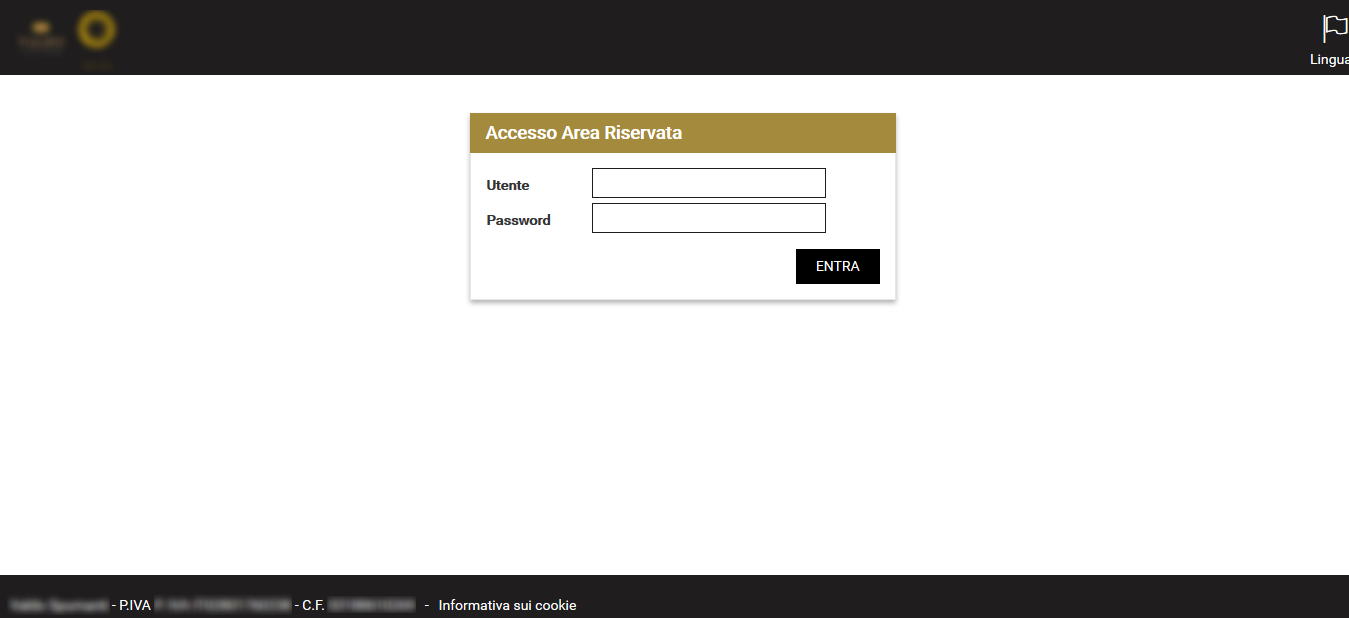
\includegraphics[width=\linewidth]{Immagini/p1/index.png}
	\caption{Pagina di accesso al portale}
	\label{fig:login1}
\end{figure}

Una nota va posta sull'utilizzo delle sessioni. La maggioranza degli oggetti caricati dalla libreria Spring Core sono configurati per essere \textit{session scope}. Questo fa sì che le istanze siano legate agli utenti che utilizzano il B2B, in modo tale da evitare possibili conflitti su nuovi ordini o clienti. Una conseguenza diretta è che non è possibile aprire due finestre dello stesso browser per accedere con utenti diversi. La sessione è inoltre impostata per scadere dopo un certo tempo di inattività, costringendo l'utente a rieffettuare il login, sia per motivi di sicurezza, sia per garantire un maggior controllo sui contenuti, impedendo di concludere operazioni su dati che potrebbero essere deprecati.

Nel corso delle settimane di stage, sono state fatte alcune implementazioni sulla base di richieste del cliente. Generalmente i lavori svolti per questo progetto erano basati su analisi effettuate precedentemente al mio arrivo, in quanto parti dei preventivi presentati al cliente. Prima di iniziare a modificare il codice, mi è tuttavia stato chiesto di presentare in forma di analisi il flusso delle operazioni necessarie per raggiungere l'obiettivo. Le richieste per questo progetto erano legate principalmente all'aggiunta o modifica di informazioni nei risultati o nei parametri di ricerca delle interrogazioni.

Vengono ora presentate alcune delle modifiche effettuate.

\subsection{Codice cliente}
Il codice cliente è un'informazione chiave nel B2B, in quanto contribuisce a costruire ed individuare gli ordini. Dal codice cliente dipendono il tipo dell'ordine, i listini, gli sconti e le promozioni. Per questo motivo poter effettuare ricerche tramite questo codice agevola gli agenti e l'amministrazione. Una delle prime richieste è stata proprio di introdurre questa informazione nei parametri e nei risultati delle interrogazioni.
\begin{figure}
	\centering
	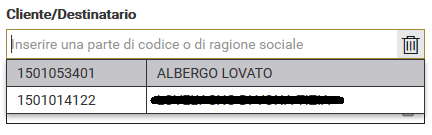
\includegraphics{Immagini/p1/clienti-params.png}
	\caption{Parametri per la ricerca dei clienti}
	\label{fig:clienti-params}
\end{figure}

Per agevolare l'utente nell'inserimento di informazioni corrette, è stato predisposto un campo di testo \virgolette{autocompletante}. Una volta digitati tre caratteri nel campo di input viene eseguita una \textit{query} di ricerca nel database per estrarre la lista dei clienti con codice o descrizione (la ragione sociale nella terminologia del gestionale) contenenti la stringa cercata. Questa \textit{query} deve essere il più ottimizzata possibile, in quanto l'utente non deve subire un rallentamento per un'azione come la ricerca, che ha come scopo quello di far raggiungere più rapidamente gli obiettivi. Un approccio alternativo poteva essere quello di caricare la lista di tutti gli utenti nel \textit{backing bean}, per poi utilizzare i metodi offerti dall'interfaccia \texttt{List} per ottenere la sottolista ricercata.

\subsection{Risultati di ricerca}
Una delle funzionalità più variabili nel B2B è l'ordinamento dei risultati di ricerca, soprattutto nella presentazione dei clienti. Oltre alle modalità di ordinamento comuni (ordine alfabetico o per codice) già predisposti da alcuni componenti Primefaces, che lavora sulle colonne, a volte sono richiesti ordinamenti più complessi.

Nella creazione dell'ordine, la scelta del cliente è solitamente il primo step. I clienti presenti nell'anagrafica sono di due tipi: clienti normali o destinatari. Questi possono poi assumere nella costruzione dell'ordine tre ruoli: cliente di fatturazione, cliente destinatario e, se entrambi i precedenti sono definiti e distinti, è possibile impostare una diversa destinazione. Nello specifico di questo progetto, l'ordinamento richiesto era il seguente: il clienti dovevano essere ordinati alfabeticamente, ma ad ognuno dovevano seguire, se presenti, le varie destinazioni. La lista di partenza era una collezione di \texttt{BusinessPartner}, recuperata direttamente dal database, indistintamente dal ruolo. Per ottenere il risultato voluto sono stati quindi utilizzati i comparatori Java, che permettono di definire per uno stesso oggetto varie regole di ordinamento, utilizzabili poi nelle funzioni di \textit{sorting} offerte dalle collezioni. 
Il risultato è presentato in \hyperref[fig:listaclienti]{figura \ref{fig:listaclienti}}.
\begin{figure}
	\centering
	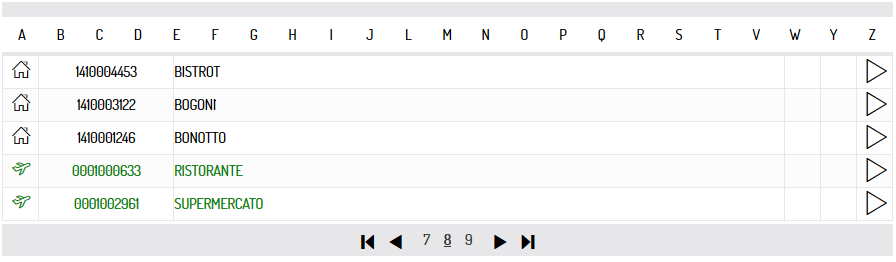
\includegraphics[width=\linewidth]{Immagini/p1/lista-clienti.png}
	\caption{Scelta del cliente nella creazione dell'ordine}
	\label{fig:listaclienti}
\end{figure}

Per rendere più utilizzabile e più accessibile i risultati proposti, questi sono paginati. Primefaces permette di definire il numero di risultati da presentare a priori, indipendentemente dal dispositivo, o dinamicamente, adattando il numero alle dimensioni dello schermo. Questo comportamento dinamico può risultare un vantaggio, in quanto permette di visualizzare il B2B come schermata unica, evitando eventuali scroll che possono nascondere informazioni importanti all'utente, ma anche uno svantaggio, in quanto con dispositivi piccoli e centinaia di risultati possono essere create migliaia di pagine con poche righe; un risultato non proprio efficiente. Per questo motivo per dispositivi come i tablet viene solitamente prefissato il numero di risultati da mostrare.

\subsection{Agenda}
In portali come il B2B, dove sono presenti molte funzionalità, tutte collegate tra loro, il numero di passaggi per completare determinate azioni è importante: per facilitare l'utente nel passaggio tra funzioni diverse è possibile inserire collegamenti tra essi, che riassumano una serie di click altrimenti a carico dell'utente. Uno di questi casi è la creazione di appuntamenti.

In questo progetto è stata richiesta la possibilità di crearli direttamente dalla scheda del cliente, impostando già alcuni parametri per l'evento. Sono stati quindi inseriti dei pulsanti al cui click l'utente viene portato all'agenda e viene creato un appuntamento per il cliente specifico, con la possibilità di inserire direttamente le informazioni mancanti. Una volta inserite queste, l'utente (solitamente l'agente), può salvare l'evento e tornare alla scheda del cliente, o continuare la navigazione. Con un semplice pulsante sono stati riprodotte quindi tre azioni: l'utente clicca sulla voce di menu per aprire l'agenda; l'utente clicca sul pulsante per creare un nuovo evento; l'utente seleziona il cliente desiderato dal campo di input \textit{autocomplete}. Sebbene questa possa essere una caratteristica molto semplice, il B2B è pieno di questi tipi di collegamenti, che permettono di completare attività risparmiando complessivamente molto tempo.

\section{Secondo progetto}
Il secondo progetto su cui si è incentrato lo stage fa parte della categoria dei B2B a sè stanti. Questo progetto è completamente personalizzato e ha ben poco a che fare con lo standard in produzione. Anche se le funzionalità principali sono le stesse, il modo in cui vengono presentate all'utente sono totalmente diverse. Anche graficamente, questo portale rispecchia più gli \textit{e-commerce} B2C piuttosto che gli altri B2B. Essendo così tanto personalizzato, in questo progetto emergono le problematiche analizzate in \hyperref[sec:b2b-smi]{sezione \ref{sec:b2b-smi}}, sia riguardo alla struttura, sia relativamente allo strumento di versionamento correntemente utilizzato.

\subsection{Progettazione}
Per un approccio iniziale con questo progetto il più consapevole possibile sono stati realizzati dei diagrammi delle classi personalizzate per il cliente. La \hyperref[fig:arch-p2]{figura \ref{fig:arch-p2}} rappresenta l'architettura ad alto livello tramite un diagramma dei \textit{package}.
\begin{figure}[H]
	\centering
	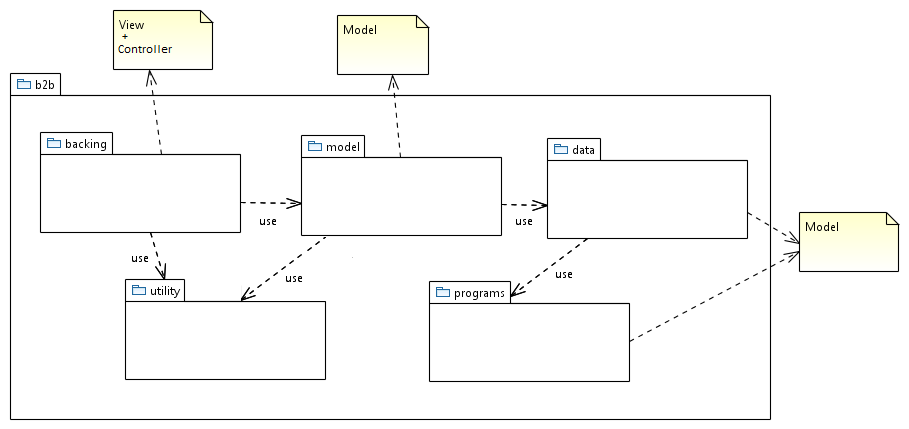
\includegraphics[width=\linewidth]{Immagini/p2/architettura.png}
	\caption{Architettura generale del secondo progetto}
	\label{fig:arch-p2}
\end{figure}

Vengono ora riportati i diagrammi delle classi per i \textit{package} dei \textit{backing bean} (\hyperref[fig:bck]{figura \ref{fig:bck}}), dei \textit{manager} (\hyperref[fig:manager]{figura \ref{fig:manager}}) e dei \textit{data provider} (\hyperref[fig:data]{figura \ref{fig:data}}). Nei diagrammi, che riportano solo le classi personalizzate, si può vedere come ogni tipo di entità abbia i corrispettivi oggetti nei vari \textit{package}. Non sono riportate le relazioni tra le classi in quanto richiederebbero un diagramma troppo grande per presentarlo in questa relazione; i seguenti hanno quindi lo scopo di mostrare applicati i concetti presentati in \hyperref[sec:b2b-struttura]{sezione \ref{sec:b2b-struttura}}.
\begin{figure}[H]
	\centering
	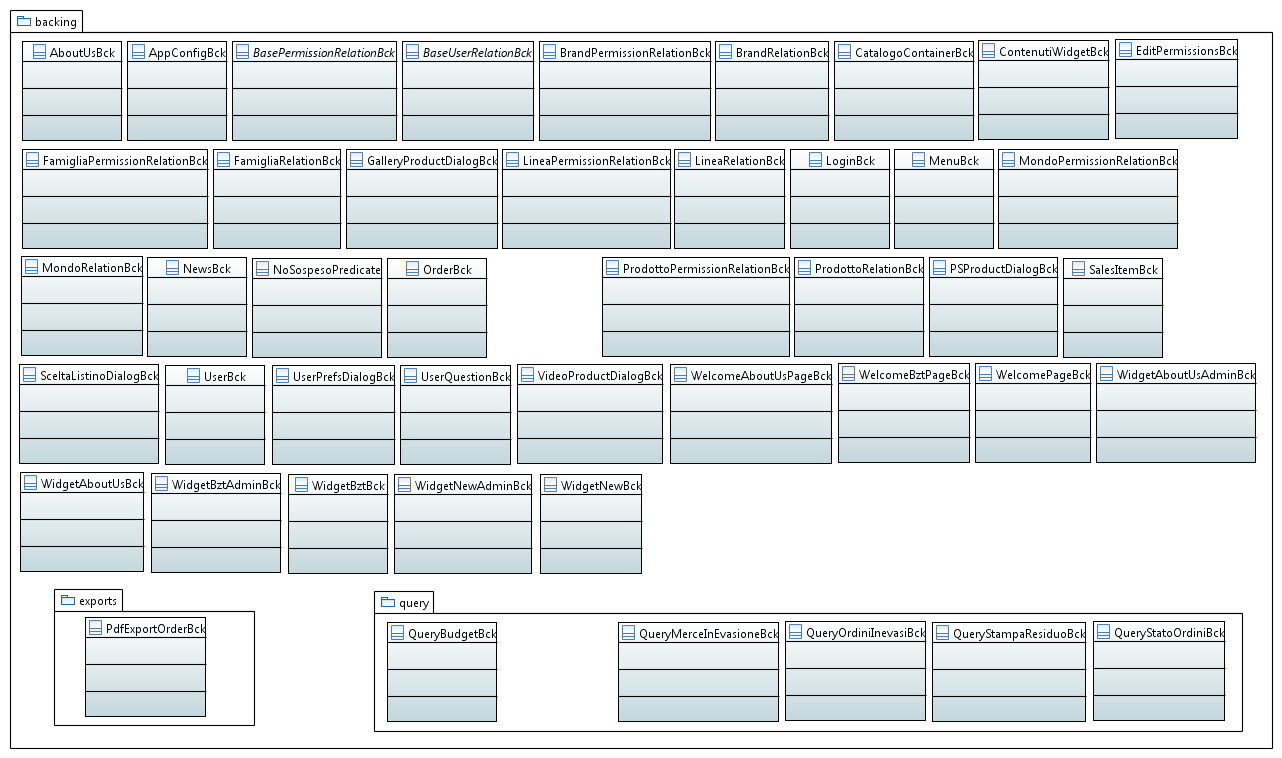
\includegraphics[height=\linewidth,angle=90]{Immagini/p2/bck.png}
	\caption{\textit{Backing bean} personalizzati}
	\label{fig:bck}
\end{figure}
\begin{figure}[H]
	\centering
	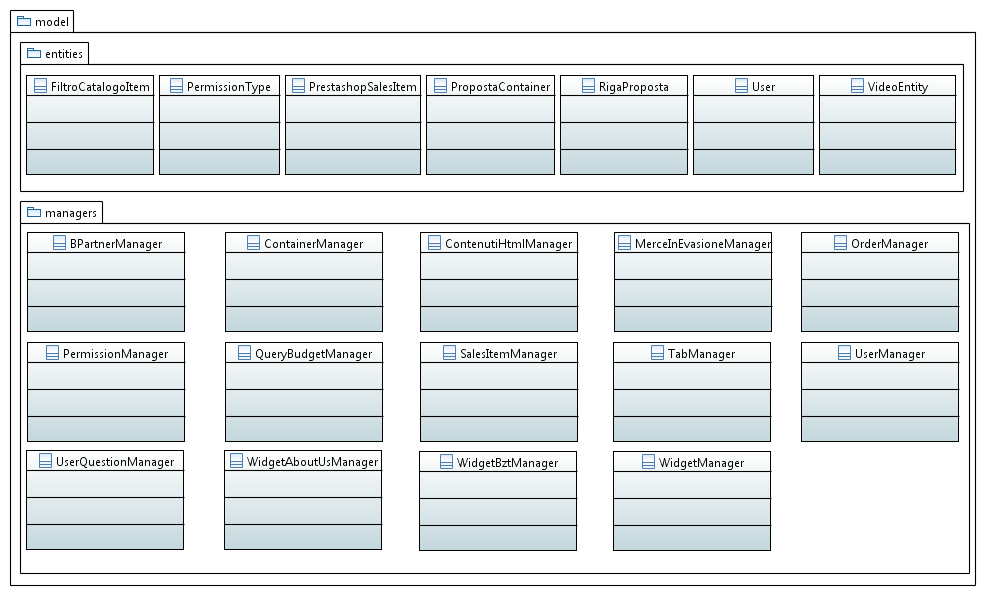
\includegraphics[height=0.9\linewidth,angle=90]{Immagini/p2/manager.png}
	\caption{\textit{Manager} e entità personalizzati}
	\label{fig:manager}
\end{figure}
\begin{figure}[H]
	\centering
	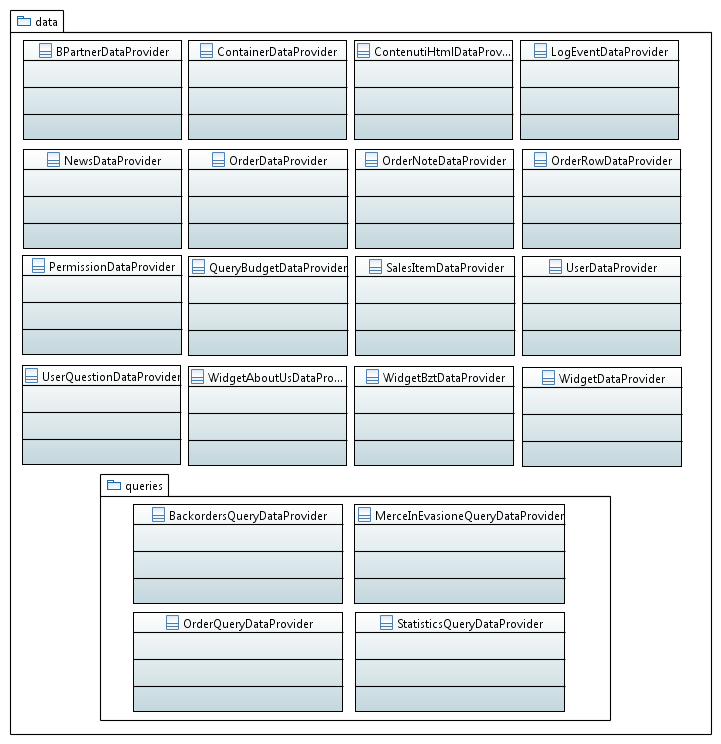
\includegraphics[width=\linewidth]{Immagini/p2/data.png}
	\caption{\textit{Data provider} personalizzati}
	\label{fig:data}
\end{figure}


\subsection{Task per invio di newsletter}
Una delle funzionalità create per questo progetto è un task per l'invio di newsletter riguardo a nuove offerte disponibili sul portale. Per realizzare questo compito è stata estesa la classe \texttt{ExtendedTask} del pacchetto standard, che si occupa di creare un thread il cui avvio è programmabile tramite interfaccia grafica. Il task si occupa di recuperare dal database le nuove proposte disponibili per tipologia, quindi carica l'elenco dei destinatari, a seconda della lingua carica e traduce il template del messaggio, lo compila con i dati corretti e infine lo invia al gruppo di destinatari il cui locale (inteso come il gruppo di parametri che definisce la lingua, il paese e qualsiasi altra variante specifica, scelti dall'utente per la visualizzazione dell'interfaccia) corrisponde alla lingua di traduzione del template.

Il recupero delle informazioni avviene anch'esso seguendo alcuni passaggi:
\begin{itemize}
	\item vengono caricate dal database tutte le proposte con data di inizio validità corrispondente al parametro di configurazione del task, settabile tramite interfaccia grafica e di default corrispondente al giorno successivo alla data di sistema;
	\item delle proposte risultanti vengono quindi caricate le immagini dei prodotti;
	\item l'elenco dei prodotti viene ordinato per tipologia.
\end{itemize}
Poiché il numero di proposte è molto variabile, il template è costruito con un unico prodotto per categoria. Questo viene poi replicato tante volte quante sono le proposte o eliminato nel caso in cui non ve ne siano. In questo caso viene eliminata anche la sezione relativa.


\subsection{Export log utenti}
Sapere cosa fanno gli utenti e quali sono le funzionalità più utilizzate sono un aspetto importante per chi gestisce il B2B, in quanto permette di favorirne l'utilizzo e quindi la soddisfazione degli utenti stessi. Inoltre, sapere quali utenti utilizzano maggiormente il portale fa sì che possano essere applicate promozioni o condizioni di vendita a loro mirate. L'utilizzo di log per gli eventi che riguardano gli utenti è quindi un vantaggio notevole per l'amministrazione, che grazie ad essi ha un nuovo modo di conoscere i propri agenti e clienti, oltre che tramite gli ordini effettuati.

L'analisi di questo tipo di dati è effettuata tramite l'esportazione dei log sotto forma di fogli di calcolo. Anche in questo caso sono disponibili vari parametri di ricerca per risultati più precisi, come ad esempio il tipo di evento, il nome utente, le date di inizio e fine periodo. Viene anche data la possibilità di effettuare vari tipi di esportazione, a seconda del numero di dati che si vogliono avere: il riepilogo permette di tener traccia della quantità di operazioni effettuate dagli utenti, indipendentemente dalla tipologia; l'export normale comprende i tipi di operazioni e informazioni specifiche sul tipo di operazione, come ad esempio lo \textit{user agent} del browser utilizzato che, nonostante non costituisca un'informazione precisa ed assoluta, è comunque indicativa; l'export completo, infine, comprende un numero molto maggiore di informazioni, soprattutto rispetto a dati specifici degli utenti.

\subsection{Ottimizzazione query}
Allo sviluppo di questa funzionalità è seguito un lavoro di ottimizzazione delle \textit{query} presenti per il recupero dei dati dal database. In particolare, nell'esportazione dei prodotti viene creato un file contenente migliaia di elementi. La modalità con cui venivano reperiti i prodotti rendeva il processo di creazione estremamente lungo, richiedendo parecchi minuti di caricamento. L'obiettivo era quindi quello di ridurre questo tempo di esecuzione, ottimizzando sia le \textit{query} che il caricamento delle immagini. 

Il risultato è stato ottenuto limitando gli accessi alle due fonti dei dati, sfruttando i \textit{prepared statement} per creare interrogazioni che, nonostante la maggior complessità rispetto alle precedenti, con tempi di esecuzione relativi anche più lunghi, risultavano complessivamente più precise e più rapide. Allo stesso modo il caricamento delle immagini è stato reso massivo e non più a livello individuale per prodotto. Come risultato finale è stato raggiunto un dimezzamento dei tempi per la creazione del primo \textit{export}, mentre le successive richieste sono ora eseguite in pochi secondi.

\section{I due progetti a confronto}
I due progetti sono dunque molto diversi tra loro, nonostante la base sia la stessa. La prima e più evidente differenza è la grafica e ciò dipende oltre che dal tipo di prodotti anche dalla professione del personale addetto alla gestione del B2B. Mentre per il primo progetto ad occuparsi del portale è un responsabile \Gls{CED}, per il secondo progetto il referente è un grafico. Questo ha determinato un'attenzione molto maggiore ai dettagli grafici, a volte anche a scapito dell'usabilità. Vengono ora presentate alcune delle funzionalità comuni, evidenziandone le differenze.

\subsection{Ricerca interrogazioni}
Il pannello di ricerca delle interrogazioni è probabilmente l'unica cosa che i due progetti hanno in comune (\hyperref[fig:params-1]{figura \ref{fig:params-1}} e \hyperref[fig:clienti-params-2]{figura \ref{fig:clienti-params-2}}). Nel secondo progetto però vi è una divergenza nel modo in cui il componente è presentato all'interno delle varie interrogazioni. Per alcune è stato deciso di inserire le \textit{label} dopo ai campi di input (\hyperref[fig:params-2]{figura \ref{fig:params-2}}). Questo tipo di presentazione può creare confusione anche per un utilizzatore consuetudinario, che nelle altre interrogazioni, negli altri \textit{e-commerce} e in generale in qualsiasi altro sito web, è abituato a vedere le etichette descrittive sopra o a sinistra dei relativi campi.
\begin{figure}[H]
	\centering
	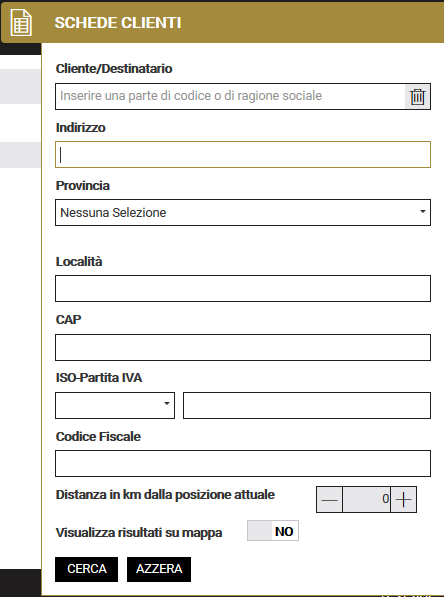
\includegraphics[height=0.8\linewidth]{Immagini/p1/params.png}
	\caption{Form di ricerca per il progetto 1}
	\label{fig:params-1}
\end{figure}
\begin{figure}[H]
	\centering
	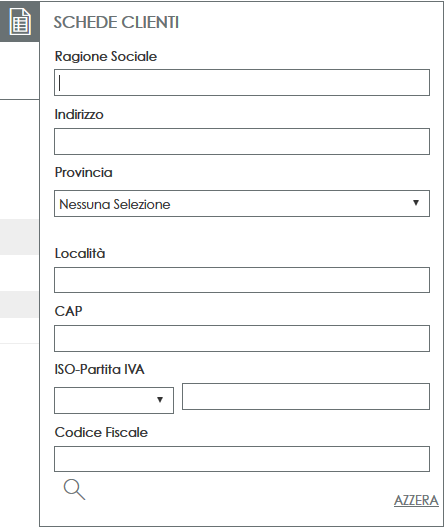
\includegraphics[height=0.7\linewidth]{Immagini/p2/clienti-params.png}
	\caption{Form di ricerca clienti per il progetto 2}
	\label{fig:clienti-params-2}
\end{figure}
\begin{figure}[H]
	\centering
	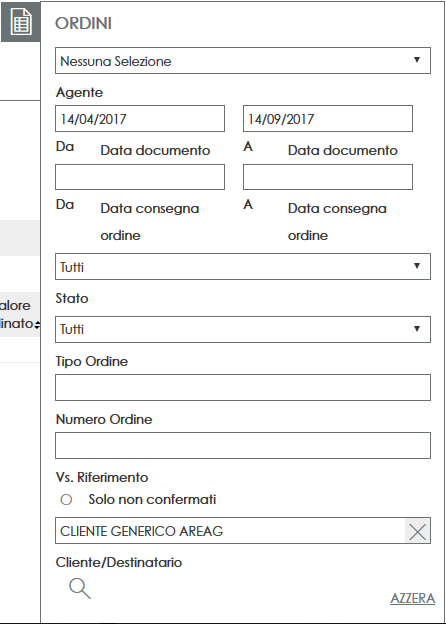
\includegraphics[height=0.8\linewidth]{Immagini/p2/params.png}
	\caption{Form di ricerca ordini per il progetto 2}
	\label{fig:params-2}
\end{figure}

\subsection{Catalogo prodotti}
Anche la presentazione dei prodotti a catalogo è nettamente differente. Per il primo progetto i prodotti sono presentati in un elenco (\hyperref[fig:catalogo-1]{figura \ref{fig:catalogo-1}}), raggruppati per categoria. Nel secondo progetto invece è stato scelto un catalogo molto più simile a quello degli \textit{e-commerce} B2C. In entrambi i progetti i prodotti sono visualizzabili anche senza aver creato un ordine. Nel secondo progetto essi sono raggruppati per categorie generiche, come \virgolette{novità} o \virgolette{outlet}e nel tipo di presentazione a griglia (\hyperref[fig:catalogo-2]{figura \ref{fig:catalogo-2}}) grande importanza è data all'immagine del prodotto, che risulta fondamentale nell'ambito di vendita del cliente, l'arredamento.
\begin{figure}[H]
	\centering
	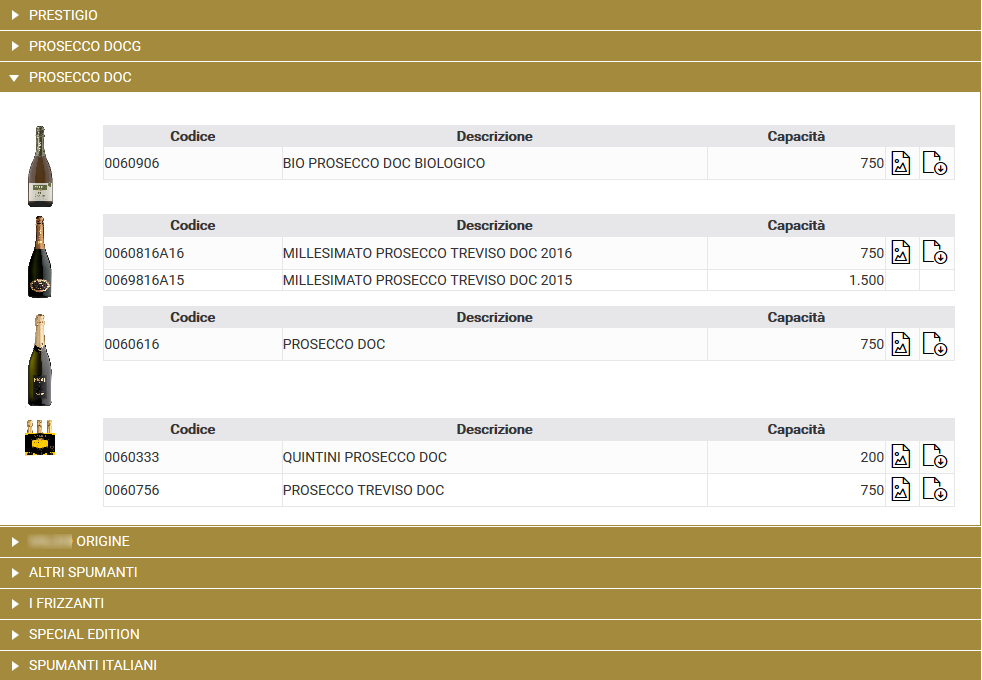
\includegraphics[width=\linewidth]{Immagini/p1/catalogo.png}
	\caption{Presentazione dei prodotti nel progetto 1}
	\label{fig:catalogo-1}
\end{figure}
\begin{figure}[H]
	\centering
	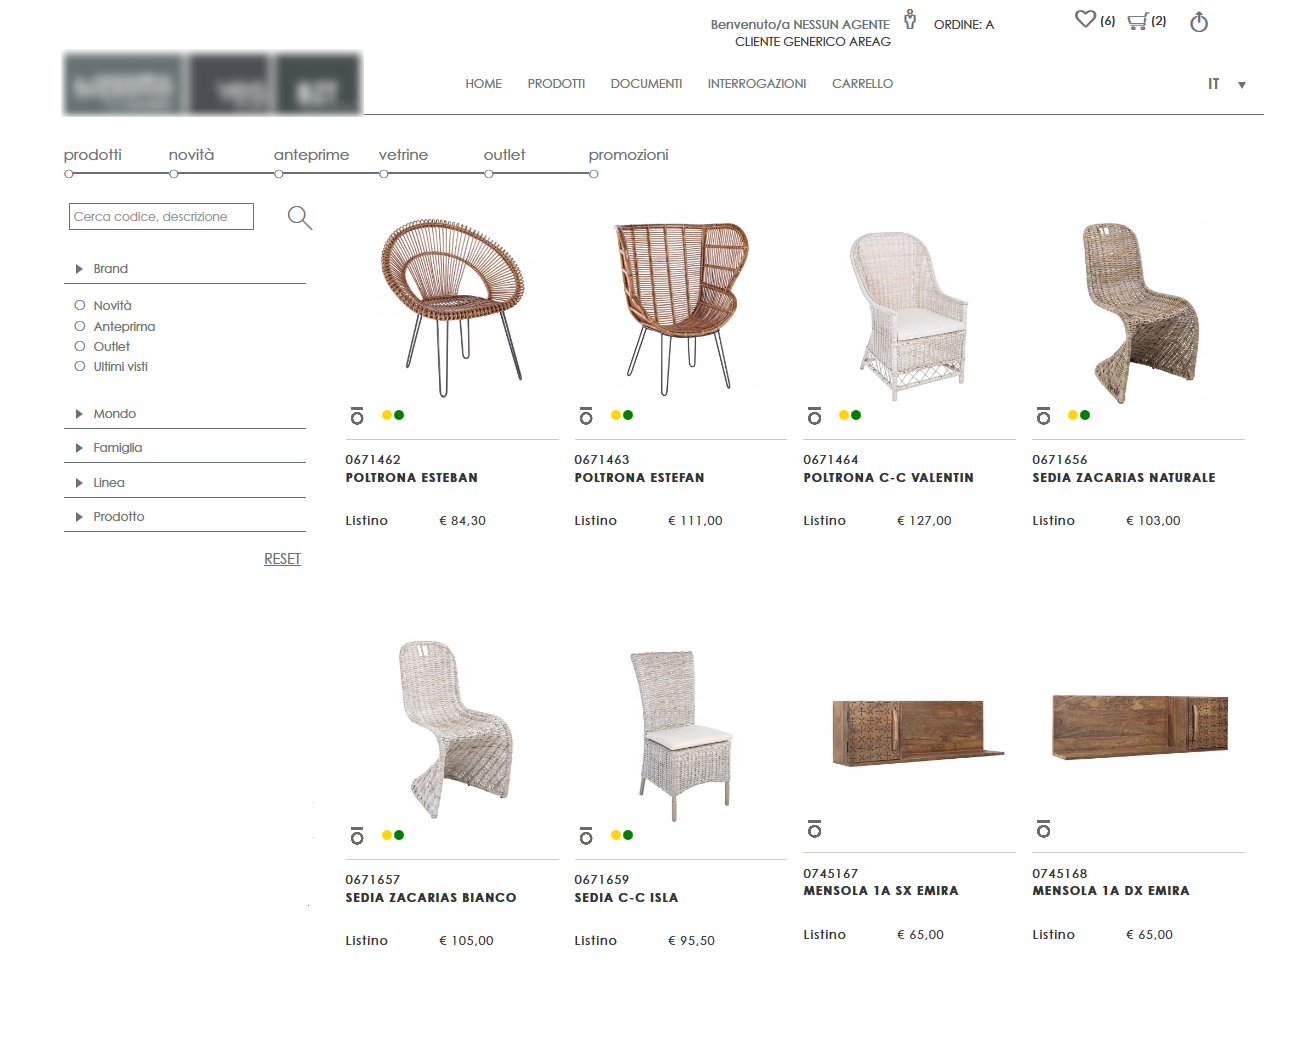
\includegraphics[width=\linewidth]{Immagini/p2/catalogo.png}
	\caption{Presentazione dei prodotti nel progetto 2}
	\label{fig:catalogo-2}
\end{figure}

\subsection{Creazione dell'ordine}
Anche il processo di creazione dell'ordine è differente per le due versioni del B2B. Nel primo progetto viene riproposto il procedimento standard, attraverso un \textit{wizard} che permette di comporre l'ordine. Ai passi standard sono aggiunti quelli personalizzati, ad esempio per l'inserimento di premi o promozioni. Nel secondo caso, invece, l'ordine prima di essere inviato è definito \virgolette{carrello}. È quindi possibile creare e gestire più carrelli contemporaneamente. Per entrambi i progetti l'ultimo step prima di confermare l'ordine e inviarlo al gestionale è il riassunto dell'ordine, un comportamento in comune anche con altri siti web e che permette all'utente di controllare le informazioni un'ultima volta. Da questa schermata è possibile anche rifinire gli ultimi dettagli.

Nonostante la funzione in comune, anche in questo caso la presentazione è totalmente differente. Nel primo progetto è stata richiesta la possibilità di inserire tutte le informazioni riguardanti il cliente di fatturazione e di spedizione prima di inviare l'ordine, tra cui il pagamento e i contatti. I dati dovevano inoltre essere compressi per rientrare in una schermata singola (sia per utilizzo tramite computer che, per quanto possibile, da tablet). Il risultato è presentato in \hyperref[fig:summary-1]{figura \ref{fig:summary-1}}.
\begin{figure}[H]
	\centering
	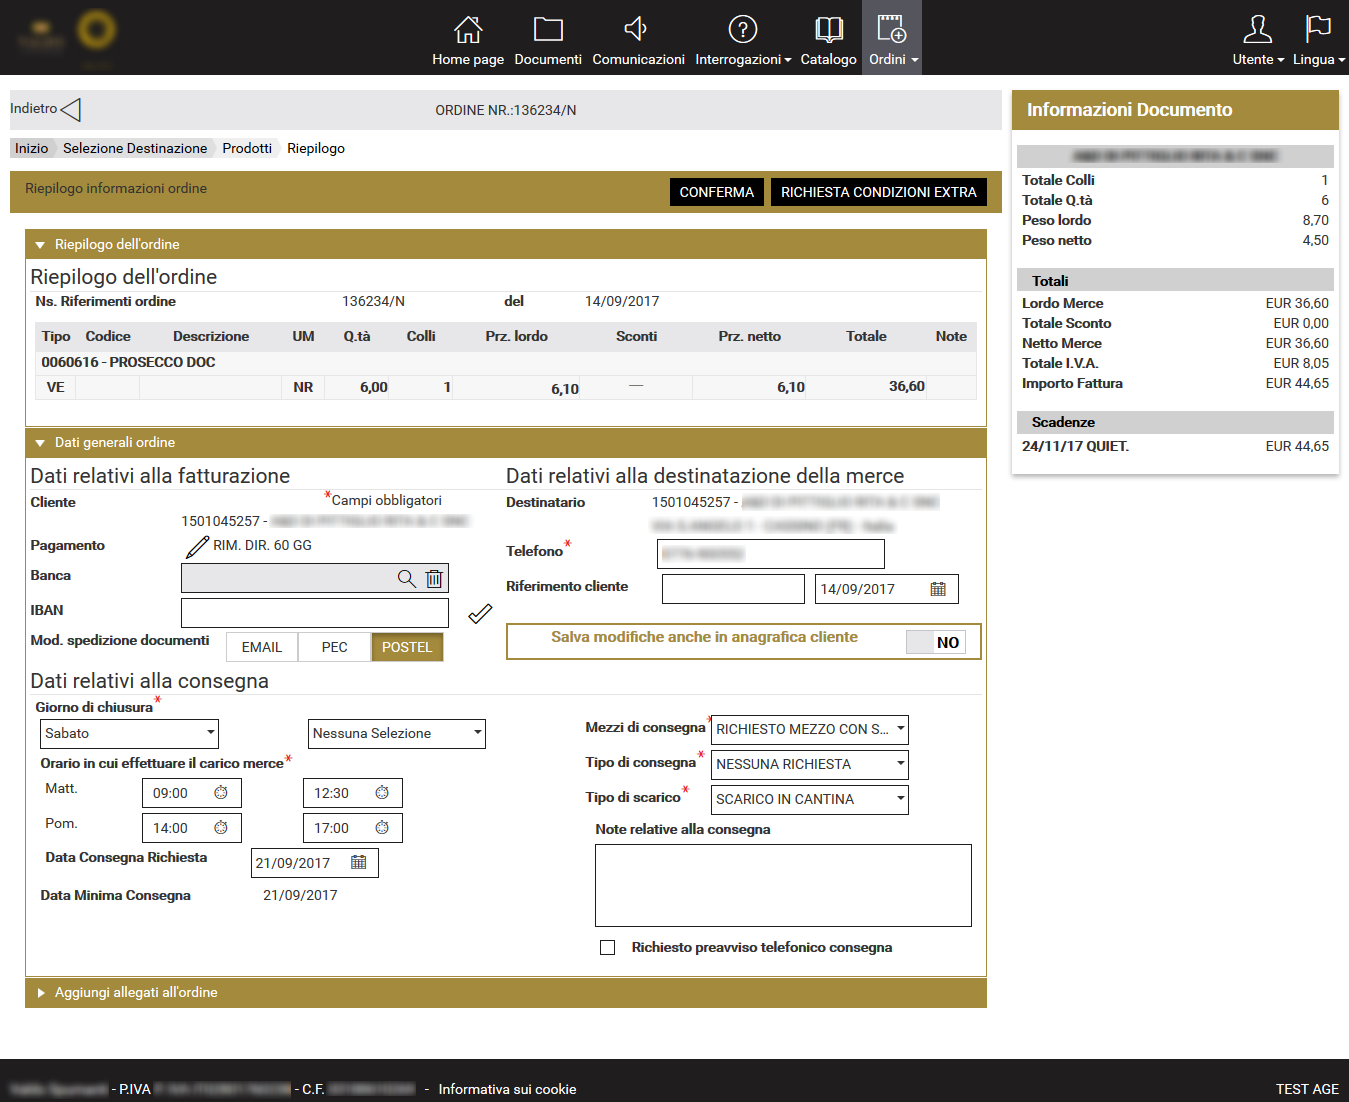
\includegraphics[width=\linewidth]{Immagini/p1/summary.png}
	\caption{Schermata riepilogativa del progetto 1}
	\label{fig:summary-1}
\end{figure}
Nel secondo progetto invece, il riepilogo dell'ordine è del tutto statico (\hyperref[fig:summary-2]{figura \ref{fig:summary-2}}). Tutte le eventuali modifiche vanno quindi effettuate tornando al carrello.
\begin{figure}[H]
	\centering
	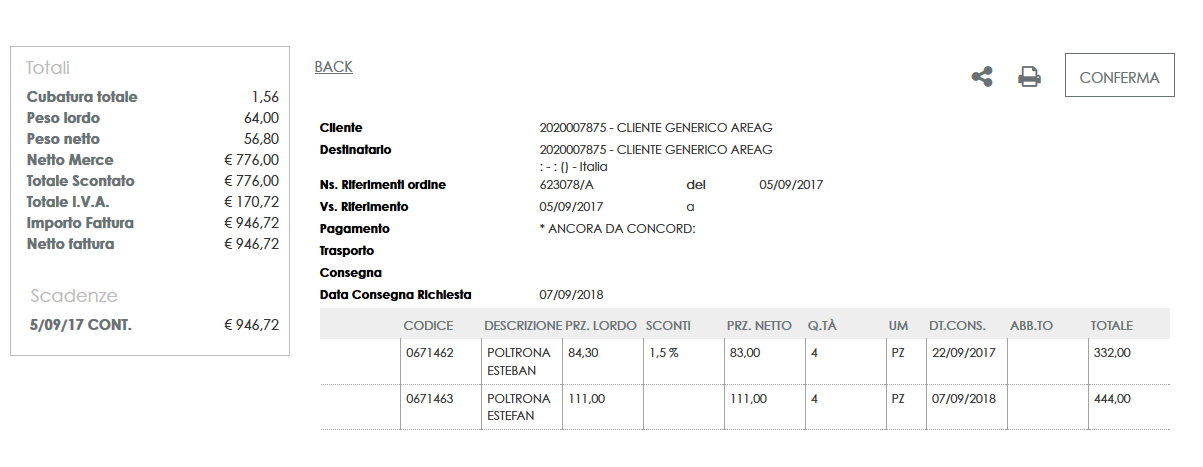
\includegraphics[width=\linewidth]{Immagini/p2/summary.png}
	\caption{Schermata riepilogativa del progetto 2}
	\label{fig:summary-2}
\end{figure}

Una nota va posta sulla pagina che permette di modificare i carrelli (\hyperref[fig:carrello-2]{figura \ref{fig:carrello-2}}), ed in particolare sulla visualizzazione dei dati di testata. I dati sono contenuti in un form, modificabile dall'utente. Il problema è che il cliente ha voluto rimuovere tutti i segnali che tali parametri sono in realtà campi di input, violando di fatto tutte le convenzioni del web. In \hyperref[fig:carrello-form]{figura \ref{fig:carrello-form}} è presentato il modulo, dove i campi editabili sono i valori della data consegna richiesta e delle note.
\begin{figure}[H]
	\centering
	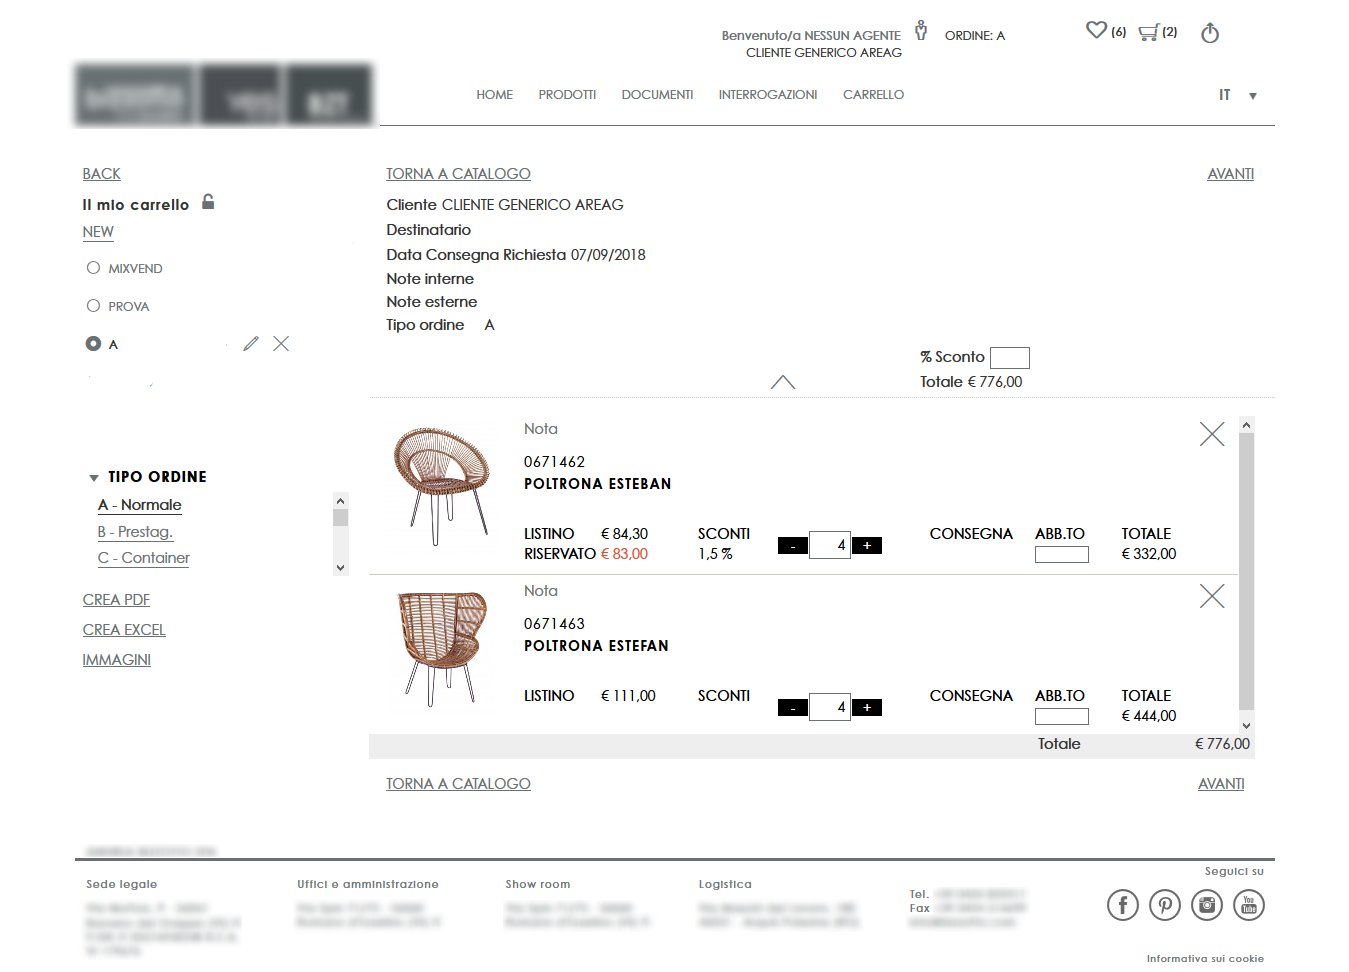
\includegraphics[width=\linewidth]{Immagini/p2/carrello.png}
	\caption{Pagina di gestione del carrello per il progetto 2}
	\label{fig:carrello-2}
\end{figure}
\begin{figure}[H]
	\centering
	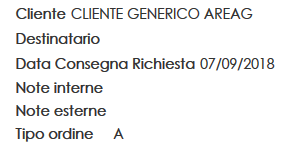
\includegraphics[width=0.5\linewidth]{Immagini/p2/carrello-form.png}
	\caption{Form di modifica dei dati di testata dell'ordine}
	\label{fig:carrello-form}
\end{figure}
	\chapter{Conclusioni}
  
	
	%----------------------------------------------------------------------------------------
	%	THESIS CONTENT - APPENDICES
	%----------------------------------------------------------------------------------------
	
	\appendix % Cue to tell LaTeX that the following "chapters" are Appendices
	
	% Include the appendices of the thesis as separate files from the Appendices folder
	% Uncomment the lines as you write the Appendices
	\chapter{Applicazioni web JavaEE}\label{app:javaee}
\begin{flushright}
	\parbox{13cm}{\small In questa appendice viene presentata la struttura di un'appilcazione web JavaEE, descrivendone le componenti ed il loro funzionamento. In particolare, viene descritto il funzionamento della servlet FacesServlet.}
\end{flushright}
	%\include{Appendices/AppendixB}
	%\include{Appendices/AppendixC}
	
	\printglossary[type=\acronymtype, title=Acronimi, nonumberlist]
	\printglossary[title=Glossario, nonumberlist]
	
	%----------------------------------------------------------------------------------------
	%	BIBLIOGRAPHY
	%----------------------------------------------------------------------------------------
	
	\printbibliography[heading=bibintoc]
	

	%----------------------------------------------------------------------------------------
	
	
\end{document}
